\chapter{Spin e sistemi a più corpi}

\section{Prodotto tensore}
\lezione{20}{12/11/2025}

Consideriamo due sistemi quantistici indipendenti, descritti dai rispettivi spazi di Hilbert: \(S_1\to \mathcal{H}_1\) e \(S_2\to \mathcal{H}_2\)
come possiamo descrivere un sistema \(S = S_1 \cup S_2\) unione dei due sottosistemi?

\begin{definition}
    Dati due spazi di Hilbert \(\mathcal{H}_1\) e \(\mathcal{H}_2\), il loro \textit{prodotto tensore} è un nuovo spazio di Hilbert \(\mathcal{H} = \mathcal{H}_1 \otimes \mathcal{H}_2\).
    Esso è definito dall'operazione di prodotto tensore \(\otimes\), che associa a ogni coppia di vettori \(\ket{\Psi_1} \in \mathcal{H}_1\) e \(\ket{\Psi_2} \in \mathcal{H}_2\) un vettore \(\ket{\Psi_1} \otimes \ket{\Psi_2} \in \mathcal{H}\), con le seguenti proprietà:
    \begin{itemize}
        \item \textbf{Bilinearità:} L'operazione è lineare in ciascun argomento. Per ogni \(\lambda \in \mathbb{C}\):
        \begin{align*}
            (\lambda \ket{\Psi_1}) \otimes \ket{\Psi_2} &= \ket{\Psi_1} \otimes (\lambda \ket{\Psi_2}) = \lambda (\ket{\Psi_1} \otimes \ket{\Psi_2}) \\
            (\ket{\Psi_1} + \ket{\chi_1}) \otimes \ket{\Psi_2} &= \ket{\Psi_1} \otimes \ket{\Psi_2} + \ket{\chi_1} \otimes \ket{\Psi_2} \\
            \ket{\Psi_1} \otimes (\ket{\Psi_2} + \ket{\chi_2}) &= \ket{\Psi_1} \otimes \ket{\Psi_2} + \ket{\Psi_1} \otimes \ket{\chi_2}
        \end{align*}
        \item \textbf{Prodotto Scalare:} Il prodotto scalare su \(\mathcal{H}\) è definito da:
        \begin{equation}
            \braket{\Psi_1 \otimes \Psi_2}{\chi_1 \otimes \chi_2} = \braket{\Psi_1}{\chi_1}_{\mathcal{H}_1} \braket{\Psi_2}{\chi_2}_{\mathcal{H}_2}
        \end{equation}
        \item \textbf{Base Ortonormale:} Se \(\{\ket{e_{1,n}}\}\) e \(\{\ket{e_{2,m}}\}\) sono basi ortonormali di \(\mathcal{H}_1\) e \(\mathcal{H}_2\), allora l'insieme
        \begin{equation}
            \left\{ \ket{e_{1,n}} \otimes \ket{e_{2,m}} \right\}
        \end{equation}
        forma una base ortonormale di \(\mathcal{H} = \mathcal{H}_1 \otimes \mathcal{H}_2\). La dimensione dello spazio prodotto è \(\dim(\mathcal{H}) = \dim(\mathcal{H}_1) \cdot \dim(\mathcal{H}_2)\).
    \end{itemize}
\end{definition}
Dati due vettori generici \(\ket{\Psi_1} \in \mathcal{H}_1\) e \(\ket{\Psi_2} \in \mathcal{H}_2\) che si decompongono nelle rispettive basi ortonormali:
\[
    \ket{\Psi_1} = \sum_{n} a_n \ket{e_{1,n}} \qquad \ket{\Psi_2} = \sum_{m} b_m \ket{e_{2,m}}
\]
Il prodotto tensore \(\ket{\Psi_1} \otimes \ket{\Psi_2} \in \mathcal{H}_1 \otimes \mathcal{H}_2\) (con base \(\{\ket{e_{1,n}} \otimes \ket{e_{2,m}}\}\)) si scompone come:
\[
    \ket{\Psi_1} \otimes \ket{\Psi_2} = \sum_{n,m} a_n b_m \ket{e_{1,n}} \otimes \ket{e_{2,m}}
\]
Un generico vettore \(\ket{\Psi} \in \mathcal{H}\) è una combinazione lineare degli elementi della base:
\[
    \ket{\Psi} = \sum_{n,m} c_{n,m} \ket{e_{1,n}} \otimes \ket{e_{2,m}}
\]
\begin{attention}
    Non ogni stato \(\ket{\Psi} \in \mathcal{H}\) può essere scritto come prodotto tensore \(\ket{\Psi_1} \otimes \ket{\Psi_2}\).
\end{attention}

\begin{example}
    Siano \(\mathcal{H}_i \cong \mathbb{C}^2\) con base \(\{\ket{u_i}, \ket{v_i}\}\) per \(i=1,2\).
    Consideriamo il vettore in \(\mathcal{H}_1 \otimes \mathcal{H}_2\):
    \[
        \ket{\Psi} = \ket{u_1}\otimes\ket{u_2} + \ket{v_1}\otimes\ket{v_2}
    \]
    Verifichiamo se è possibile scomporlo come prodotto tensore di due stati (stato separabile):
    \[
        \ket{\Psi} \overset{?}{=} (\alpha\ket{u_1} + \beta\ket{v_1}) \otimes (\gamma\ket{u_2} + \delta\ket{v_2})
    \]
    Sviluppando il prodotto tensore, otteniamo:
    \[
        \ket{\Psi} = \alpha\gamma (\ket{u_1}\otimes\ket{u_2}) + \alpha\delta (\ket{u_1}\otimes\ket{v_2}) + \beta\gamma (\ket{v_1}\otimes\ket{u_2}) + \beta\delta (\ket{v_1}\otimes\ket{v_2}).
    \]
    Confrontando i coefficienti con l'espressione originale di \(\ket{\Psi}\), si ottiene il sistema di equazioni:
    \[
        \alpha\gamma = 1, \qquad \alpha\delta = 0, \qquad \beta\gamma = 0, \qquad \beta\delta = 1.
    \]
    Dalla seconda equazione, \(\alpha\delta = 0\), deve valere \(\alpha=0\) o \(\delta=0\).
    \begin{itemize}
        \item Se \(\alpha=0\), la prima equazione diventa \(\alpha\gamma = 0\), in contraddizione con \(\alpha\gamma = 1\).
        \item Se \(\delta=0\), la quarta equazione diventa \(\beta\delta = 0\), in contraddizione con \(\beta\delta = 1\).
    \end{itemize}
    In entrambi i casi si giunge a una contraddizione, dunque non è possibile scomporlo. 
\end{example}


\subsection{Operatori in \texorpdfstring{\(\mathcal{H}_1\otimes\mathcal{H}_2\)}{H1⊗H2}}

Consideriamo due operatori lineari definiti sui rispettivi spazi di Hilbert:
\[
    A_1: \mathcal{H}_1 \to \mathcal{H}_1 \qquad B_2: \mathcal{H}_2 \to \mathcal{H}_2
\]

L'azione dell'operatore prodotto tensoriale \(A_1 \otimes B_2\) su un generico vettore di \(\mathcal{H}_1 \otimes \mathcal{H}_2\), espresso nella base prodotto \(\ket{e_n} \otimes \ket{u_m}\), è data da:
\begin{equation}
    (A_1 \otimes B_2) \left( \sum_{n,m} C_{n,m} \ket{e_n} \otimes \ket{u_m} \right) = \sum_{n,m} C_{n,m} (A_1\ket{e_n}) \otimes (B_2\ket{u_m})
\end{equation}
In pratica, \(A_1\) agisce sui ket \(\ket{e_n}\) (spazio \(\mathcal{H}_1\)) e \(B_2\) agisce sui ket \(\ket{u_m}\) (spazio \(\mathcal{H}_2\)).

Un operatore generico \(G: \mathcal{H} \to \mathcal{H}\) (dove \(\mathcal{H} = \mathcal{H}_1 \otimes \mathcal{H}_2\)) si può scrivere come somma di prodotti tensoriali:
\begin{equation}
    G = \sum_{n,m} C_{nm} \, A_{1,n} \otimes B_{2,m}
\end{equation}

Dati \(A_1\) su \(\mathcal{H}_1\) e \(B_2\) su \(\mathcal{H}_2\), si definiscono le loro estensioni allo spazio totale:
\begin{align}
    \tilde{A}_1 &= A_1 \otimes I_{\mathcal{H}_2} \\
    \tilde{B}_2 &= I_{\mathcal{H}_1} \otimes B_2
\end{align}
Questi operatori (che spesso vengono indicati senza tilde per abuso di notazione) rappresentano fisicamente operatori che agiscono solo su uno spazio (il proprio sottosistema), lasciando inalterato l'altro (agendo come l'identità).

\begin{remark}
    Gli operatori \(\tilde{A}_1\) e \(\tilde{B}_2\) (che non fanno niente nello spazio prodotto \(\mathcal{H}_1 \otimes \mathcal{H}_2\) dell'altro operatore) commutano sempre:
    \begin{equation}
        \tilde{A}_1 \tilde{B}_2 = A_1 \otimes B_2 = \tilde{B}_2 \tilde{A}_1
    \end{equation}
    Operatori che agiscono su spazi di Hilbert diversi (gradi di libertà distinti) commutano. Fare misure sul primo sistema senza toccare il secondo non perturba il secondo.
\end{remark}

Poiché commutano, esiste una base di autostati comune.
Siano \(A_1\) e \(B_2\) operatori autoaggiunti (a.a.) con le rispettive basi ortonormali:
\begin{itemize}
    \item Per \(\mathcal{H}_1 \ni A_1\): \(\left\{ \ket{a, r} \right\}_{\substack{a \in \sigma(A_1) \\ r=1,\dots,d(a)}}\) base O.N. di \(\mathcal{H}_1\)
    \item Per \(\mathcal{H}_2 \ni B_2\): \(\left\{ \ket{b, s} \right\}_{\substack{b \in \sigma(B_2) \\ s=1,\dots,d(b)}}\) base O.N. di \(\mathcal{H}_2\)
\end{itemize}

La base prodotto:
\begin{equation}
    \left\{ \ket{a, r} \otimes \ket{b, s} \right\}_{\substack{r=1\dots d(a) \\ s=1\dots d(b)}}
\end{equation}
è una base ortonormale di \(\mathcal{H}_1 \otimes \mathcal{H}_2\) ed è una base di autovettori simultanei di \(\tilde{A}_1\) e \(\tilde{B}_2\).

La degenerazione degli autovalori congiunti è data dal prodotto delle degenerazioni:
\[
    \deg(a, b) = d(a)\,d(b)
\]

\begin{example}[Sistema di due particelle senza spin 3D]
    
Consideriamo un sistema composto da due particelle senza spin in tre dimensioni (3D).
Lo spazio di Hilbert di ciascuna particella è:
\[
    \mathcal{H}_1 = L_2(\mathbb{R}^3, \dd[3]{\vec{x}_1}), \qquad \mathcal{H}_2 = L_2(\mathbb{R}^3, \dd[3]{\vec{x}_2}).
\]
Lo spazio di Hilbert del sistema composto è dato dal prodotto tensoriale degli spazi individuali:
\[
    \mathcal{H} = \mathcal{H}_1 \otimes \mathcal{H}_2 \cong L_2(\mathbb{R}^6, \dd[3]{\vec{x}_1} \dd[3]{\vec{x}_2}).
\]
Lo stato del sistema è descritto da una \textit{funzione d'onda a due corpi} \(\Psi(\vec{x}_1, \vec{x}_2)\), che dipende dalle coordinate di entrambe le particelle.
La condizione di normalizzazione è:
\[
    \norm{\Psi}^2 = \int_{\mathbb{R}^6} \dd[3]{\vec{x}_1} \dd[3]{\vec{x}_2} \, \abs{\Psi(\vec{x}_1, \vec{x}_2)}^2 < +\infty.
\]
La funzione d'onda è ottenuta proiettando lo stato \(\ket{\Psi}\) sulla base di posizione generalizzata \(\left\{ \ket{\vec{x}_1, \vec{x}_2} \equiv \ket{\vec{x}_1} \otimes \ket{\vec{x}_2} \right\}\):
\[
    \Psi(\vec{x}_1, \vec{x}_2) = \braket{\vec{x}_1, \vec{x}_2}{\Psi}.
\]
La densità di probabilità di trovare simultaneamente la particella 1 in un intorno di \(\vec{x}_1\) e la particella 2 in un intorno di \(\vec{x}_2\) è data da \(\abs{\Psi(\vec{x}_1, \vec{x}_2)}^2\).

Un caso particolare è quello degli \textit{stati fattorizzabili} (o separabili), in cui lo stato del sistema composto è il prodotto tensoriale di due stati puri individuali:
\[
    \ket{\Psi} = \ket{\Psi_1} \otimes \ket{\Psi_2}
\]
A questo stato fattorizzato è associata una funzione d'onda che è il semplice prodotto delle funzioni d'onda individuali:
\[
    \Psi(\vec{x}_1, \vec{x}_2) = \braket{\vec{x}_1}{\Psi_1} \braket{\vec{x}_2}{\Psi_2} = \Psi_1(\vec{x}_1) \Psi_2(\vec{x}_2).
\]
\end{example}

\begin{example}
    \[
        L_2(\mathbb{R}^3, \dd[3]{x}) \cong L_2(\mathbb{R}, \dd{x}) \otimes L_2(\mathbb{R}, \dd{y}) \otimes L_2(\mathbb{R}, \dd{z})
        \cong L_2([0,+\infty), r^2 \dd{r}) \otimes L_2(S^2, \sin\vartheta \, \dd{\vartheta} \, \dd{\varphi})    
    \]
\end{example}

\section{Spin}

Consideriamo una particella in 3 dimensioni. Avremo sempre le osservabili posizione \(\vec{X}\) e momento \(\vec{P}\).
Definiamo il momento angolare orbitale come \(\vec{L} := \vec{X} \times \vec{P}\).

Tuttavia, in generale, il generatore delle rotazioni infinitesime \(\vec{J}\) non coincide con \(\vec{L}\). Introduciamo quindi un nuovo operatore, detto \textit{operatore di Spin}:
\begin{equation}
    \vec{S} := \vec{J} - \vec{L} 
\end{equation}
dove le componenti sono \(\vec{S} = (S_x, S_y, S_z)\).

Consideriamo l'azione di un operatore unitario di rotazione \(U(\vec{\omega}) = e^{-\frac{i}{\hbar}\vec{J}\cdot\vec{\omega}}\) su un operatore vettoriale \(\vec{X}\). 
La legge di trasformazione è:
\[
U(\vec{\omega})\vec{X}U(\vec{\omega})^\dagger = R(\vec{\omega})^{-1}\vec{X}
\]
Per rotazioni infinitesime, possiamo sviluppare l'espressione usando la rappresentazione matriciale della rotazione:
\[
R(\vec{\omega})^{-1}\vec{X} \approx \left( I_3 - \sum_j \omega_j T_j \right)\vec{X}
\]
Dalla relazione tra trasformazioni infinitesime e commutatori, otteniamo:
\[
[J_j, X_k] = i\hbar \pdv{}{\omega_j} \left( R(\vec{\omega})^{-1}\vec{X} \right)_k \bigg|_{\vec{\omega}=0} = i\hbar \sum_l \epsilon_{jkl} X_l
\]
Notiamo che questa relazione di commutazione è identica a quella del momento angolare orbitale \(\vec{L}\), poiché \(\vec{X}\) si trasforma come un vettore sotto rotazioni spaziali:
\[
[J_j, X_k] = [L_j, X_k] = i\hbar \sum_l \epsilon_{jkl} X_l
\]
Analogamente, poiché anche \(\vec{P}\) e \(\vec{L}\) sono vettori, valgono le stesse relazioni:
\[
[J_j, P_k] = i\hbar \sum_l \epsilon_{jkl} P_l = [L_j, P_k]
\]
\[
[J_j, L_k] = i\hbar \sum_l \epsilon_{jkl} L_l = [L_j, L_k]
\]

Date queste relazioni, possiamo determinare i commutatori dello spin \(\vec{S} = \vec{J} - \vec{L}\) con le osservabili spaziali:

\begin{equation}
    [S_i, X_k] = [J_i - L_i, X_k] = [J_i, X_k] - [L_i, X_k] = 0
\end{equation}
\begin{equation}
    [S_i, P_k] = [J_i - L_i, P_k] = 0
\end{equation}
\begin{equation}
    [S_i, L_k] = [J_i - L_i, L_k] = 0
\end{equation}

Lo spin \(\vec{S}\) è quindi un momento angolare che commuta con tutte le variabili cinematiche spaziali (\(\vec{X}, \vec{P}, \vec{L}\)).\\
Imponendo le regole di commutazione al momento angolare totale \(\vec{J} = \vec{L} + \vec{S}\):
\[
[L_i + S_i, L_j + S_j] = i\hbar \sum_k \epsilon_{ijk} (L_k + S_k)
\]
Espandendo e semplificando i termini orbitali \([L_i, L_j]\) presenti in ambo i membri:
\[
[L_i, L_j] + [S_i, S_j] = i\hbar \sum_k \epsilon_{ijk} L_k + i\hbar \sum_k \epsilon_{ijk} S_k
\]
Si ottiene la relazione fondamentale per lo spin:
\begin{equation}
    [S_i, S_j] = i\hbar \sum_k \epsilon_{ijk} S_k
\end{equation}



Consideriamo una singola particella quantistica. Introduciamo un nuovo operatore, il momento angolare di spin, per il quale vale il seguente postulato.

\begin{postulato8}
    Per una singola particella quantistica, l'operatore \(\vec{S}^2\) ha un singolo autovalore dato da:
    \begin{equation}
        \vec{S}^2 = \hbar^2 s(s+1) I
    \end{equation}
    dove \(s \in \frac{1}{2}\mathbb{N}\) è un numero quantico caratteristico: ogni singola particella quantistica ha un singolo valore di \(s\) fissato.
\end{postulato8}

L'insieme di operatori \(\left\{ X_1, X_2, X_3, \vec{S}^2, S_z \right\}\) commuta e costituisce un I.C.O.C. (vedi \ref{def: icoc}).
\begin{remark}
    Includere o meno \(\vec{S}^2\) nell'I.C.O.C. non cambia la sostanza, poiché tale operatore è proporzionale all'identità ed è quindi già non degenere.
\end{remark}


Ci chiediamo ora come sia strutturato lo spazio di Hilbert \(\mathcal{H}\) per una particella dotata di spin.
Rispetto al caso senza spin, abbiamo nuovi gradi di libertà. Lo spazio totale assume la forma di un \textbf{prodotto tensore} tra la parte spaziale (senza spin, \(L_2(\mathbb{R}^3, \dd[3]{x})\)) e la parte di spin:
\begin{equation}
    \mathcal{H} = \mathcal{H}_{\vec{x}} \otimes \mathcal{H}_s
\end{equation}

Gli operatori posizione \(\vec{X}\) e momento \(\vec{P}\) agiscono solo su \(\mathcal{H}_{\vec{x}}\). Nello spazio totale si scrivono come:
\[
    \vec{X} = \vec{X}_{\vec{x}} \otimes I_{\mathcal{H}_s}
\]
\[
    \vec{P} = \vec{P}_{\vec{x}} \otimes I_{\mathcal{H}_s}
\]
dove \(I_{\mathcal{H}_s}\) è l'identità nello spazio dello spin (questi operatori "non fanno nulla" nello spazio \(\mathcal{H}_s\)).

Analogamente, i 3 operatori di spin agiscono solo su \(\mathcal{H}_s\):
\[
    \vec{S} = I_{\mathcal{H}_{\vec{x}}} \otimes \vec{S}_s
\]

Poiché \(\vec{S}^2 \propto I\), è necessario utilizzare \(S_z\) come osservabile per completare l'I.C.O.C. nel sottospazio dello spin. Lo spettro di \(S_z\) è dato da:
\begin{equation}
    \sigma(S_z) = \left\{ m\hbar \right\}_{m \in \{-s, \dots, s\}}
\end{equation}
Essendo \(m\) il numero quantico magnetico che varia a passi interi da \(-s\) a \(s\), la dimensione dello spazio di Hilbert dello spin è finita e vale:
\begin{equation}
    \dim \mathcal{H}_s = 2s+1
\end{equation}

\begin{example}
    Riportiamo i valori di spin per alcune particelle note:
    \begin{itemize}
        \item Elettrone, protone, neutrone: \( s = \frac{1}{2} \)
        \item Fotone, \( W \), \( Z \): \( s = 1 \)
        \item \( \pi \), \( K \), Higgs: \( s = 0 \)
    \end{itemize}
\end{example}


% 21 Lezione del 14/11/2025

\subsection{Spin 1/2 e matrici di Pauli}
\lezione{21}{14/11/2025}

Concentriamoci ora su particelle da spin \(s = \frac{1}{2}\), avremo dunque \(\vec{S}^2= \frac{3}{4}\hbar^2 I\) , \(m = \left\{ -\frac{1}{2},\frac{1}{2} \right\}\) e lo spazio di Hilbert dello spin \(\mathcal{H}_s \cong\mathbb{C}^2\).\\
Gli autostati di \(S_z\) sono:
\[
    S_z\ket{+}=+ \frac{\hbar}{2} \ket{+} \qquad S_z\ket{-}=-\frac{\hbar}{2} \ket{-}
\]
Abbiamo perciò una base ON \(\left\{ \ket{+},\ket{-} \right\}\). Gli operatori \(S_+\) e \(S_-\) agiscono come:
\[
    S_+\ket{+}=0 \qquad S_+\ket{-}= \hbar\ket{+}
\]
\[ 
    S_-\ket{-}=0 \qquad S_-\ket{+}= \hbar\ket{-}
\]
Essendo \(\mathcal{H}_s \cong\mathbb{C}^2\), possiamo scrivere gli operatori come matrici sui numeri complessi 2x2:

\[
\ket{+} = \begin{pmatrix} 1 \\ 0 \end{pmatrix}
\qquad
\ket{-} = \begin{pmatrix} 0 \\ 1 \end{pmatrix}
\]
\[
S_z = \begin{pmatrix}
    \hbar/2 & 0 \\
    0 & -\hbar/2
\end{pmatrix}
\qquad
S_+ = \hbar \begin{pmatrix}
    0 & 1 \\
    0 & 0
\end{pmatrix}
\qquad
S_- = \hbar \begin{pmatrix}
    0 & 0 \\
    1 & 0
\end{pmatrix}
\]
Possiamo quindi scrivere le tre componenenti dello spin \(\vec{S}\) come:
\[
    S_x = \frac{S_+ + S_-}{2} = \frac{\hbar}{2}\begin{pmatrix} 0 & 1 \\ 1 & 0 \end{pmatrix}
    \qquad
    S_y = \frac{\hbar}{2} \begin{pmatrix} 0 & -i \\ i & 0 \end{pmatrix}
    \qquad
    S_z = \frac{\hbar}{2} \begin{pmatrix} 1 & 0 \\ 0 & -1 \end{pmatrix}
\]
\begin{definition}
    Definiamo così le \textit{matrici di Pauli} \(\sigma_k\) tali che \(S_k= \frac{h}{2} \sigma_k\).
    \[
        \sigma_x = \sigma_1=\begin{pmatrix}
            0 & 1\\
            1 & 0
        \end{pmatrix}
        \qquad
        \sigma_y =\sigma_2= \begin{pmatrix}
            0 & -i\\
            i & 0
        \end{pmatrix}
        \qquad
        \sigma_z =\sigma_3= \begin{pmatrix}
            1 & 0\\
            0 & -1
        \end{pmatrix}
    \]
\end{definition}

Le matrici di Pauli hanno le seguenti proprietà:
\begin{multicols}{2}
\begin{itemize}
    \item \(\sigma_k^\dagger = \sigma_k\)
    \item \(\sigma_k^2= I\)
    \item \(\sigma_k^\dagger = \sigma_k^{-1}\)
    \item se \(i \neq j, \quad \sigma_i\sigma_j=i \sum_{k}\epsilon_{ijk}\sigma_k\)
    \item \(\left[ \sigma_i, \sigma_j \right]=2i\sum_k\epsilon_{ijk}\sigma_k\)
    \item \(\left\{ \sigma_i,\sigma_j \right\}= 2\delta_{ij}I\)
    \item \(\Tr(\sigma_k)=0\)
    \item \(\det\sigma_k= -1\)
\end{itemize}    
\end{multicols}

Ogni matrice 2x2 hermitiana si scrive:
\[
    \begin{pmatrix}
        a & b-ic \\
        b+ic & d
    \end{pmatrix}
    = \frac{a+d}{2} I + b \sigma_1 + c \sigma_2 + \frac{a-d}{2} \sigma_3, \quad a,b,c,d \in \mathbb{R}
\]


Se vogliamo descrivere lo spin in una generica direzione dello spazio 3D, consideriamo un versore $\hat{n}$:
\[
\hat{n} = (n_1, n_2, n_3) \in \mathbb{R}^3, \quad \abs{\hat{n}}=1 \implies \sum_k n_k^2 = 1
\]
Definiamo la combinazione lineare delle matrici di Pauli $\sigma_k$ lungo la direzione $\hat{n}$:
\begin{equation}
    \hat{n} \cdot \vec{\sigma} := \sum_k n_k \sigma_k =
    \begin{pmatrix}
    n_3 & n_1 - i n_2 \\
    n_1 + i n_2 & -n_3
    \end{pmatrix}
\end{equation}
Calcoliamo il quadrato dell'operatore $(\hat{n} \cdot \vec{\sigma})$:
\[
(\hat{n} \cdot \vec{\sigma})^2 = \sum_{k} n_k^2 \sigma_k^2+ \sum_{i < j} n_i n_j \{\sigma_i, \sigma_j\}=I
\]
Dati due vettori generici $\vec{u}, \vec{v} \in \mathbb{R}^3$, vogliamo calcolare il prodotto delle loro contrazioni con le matrici di Pauli:
\[
(\vec{v} \cdot \vec{\sigma})(\vec{u} \cdot \vec{\sigma}) = \sum_{i,j} v_i u_j \sigma_i \sigma_j = \sum_{i,j} v_i u_j \left(\delta_{ij}I + i \sum_k \epsilon_{ijk}\sigma_k\right)
\]
Il primo termine restituisce il prodotto scalare, il secondo (antisimmetrico) restituisce il prodotto vettoriale:
\begin{equation}
(\vec{v} \cdot \vec{\sigma})(\vec{u} \cdot \vec{\sigma}) = (\vec{v} \cdot \vec{u}) I + i (\vec{v} \times \vec{u}) \cdot \vec{\sigma}
\end{equation}


Vogliamo trovare la forma esplicita dell'operatore unitario di rotazione \(U(\vec{\omega})\):
\[
    U(\vec{\omega}) = e^{-\frac{i}{\hbar}\vec{\omega}\cdot\vec{S}}
    = e^{-\frac{i}{\hbar}\frac{\hbar}{2}\vec{\omega}\cdot\vec{\sigma}} = e^{-\frac{i}{2}\vec{\omega}\cdot\vec{\sigma}}
\]
Parametrizziamo il vettore di rotazione \(\vec{\omega}\) con un asse (versore \(\hat{n}\)) e un angolo \(\theta\):
\[
    \vec{\omega} = \theta \hat{n}, \qquad \text{con } \abs{\hat{n}}=1.
\]
L'espressione diventa quindi:
\[
    U(\theta \hat{n}) = e^{-\frac{i}{2}\theta (\hat{n}\cdot\vec{\sigma})}.
\]
Per calcolare l'esponenziale, sfruttiamo la proprietà \((\hat{n}\cdot\vec{\sigma})^2 = I\),
espandiamo l'esponenziale in serie di Taylor e separiamo i termini pari e dispari:
\begin{align*}
    U(\theta\hat{n}) &= \sum_{k=0}^{\infty} \frac{1}{(2k)!} \left(-\frac{i\theta}{2}\right)^{2k} (\hat{n}\cdot\vec{\sigma})^{2k} + \sum_{k=0}^{\infty} \frac{1}{(2k+1)!} \left(-\frac{i\theta}{2}\right)^{2k+1} (\hat{n}\cdot\vec{\sigma})^{2k+1} \\
    &= \sum_{k=0}^{\infty} \frac{(-1)^k}{(2k)!} \left(\frac{\theta}{2}\right)^{2k} I - i \sum_{k=0}^{\infty} \frac{(-1)^k}{(2k+1)!} \left(\frac{\theta}{2}\right)^{2k+1} (\hat{n}\cdot\vec{\sigma}).
\end{align*}
Riconoscendo le serie di Taylor per il coseno e il seno, otteniamo la formula fondamentale per la rotazione dello spin:
\begin{equation}
    U(\theta \hat{n}) = \cos(\frac{\theta}{2})I - i \sin(\frac{\theta}{2}) (\hat{n}\cdot\vec{\sigma}).
\end{equation}
La sua rappresentazione matriciale è:
\[
    U(\theta\hat{n}) =
    \begin{pmatrix}
        \cos\frac{\theta}{2} - i n_3 \sin\frac{\theta}{2} & -i\sin\frac{\theta}{2}(n_1 - i n_2) \\
        -i\sin\frac{\theta}{2}(n_1 + i n_2) & \cos\frac{\theta}{2} + i n_3 \sin\frac{\theta}{2}
    \end{pmatrix}.
\]
Se effettuiamo una rotazione completa di un angolo \(\theta = 2\pi\) attorno a un asse qualsiasi:
\[
    U(2\pi \hat{n}) = \cos(\pi)I - i \sin(\pi)(\hat{n}\cdot\vec{\sigma}) = -I.
\]
Non otteniamo l'identità \(I\), ma \(-I\). Lo stato ruotato differisce da quello iniziale per una fase globale:
\[
    \ket{\Psi'} = U(2\pi\hat{n})\ket{\Psi} = -\ket{\Psi}.
\]
Questo risultato indica che la rappresentazione delle rotazioni per spin \(1/2\) è \textbf{genuinamente proiettiva} (o a due valori).
In generale, per una rotazione di un angolo \(\theta\) attorno all'asse \(z\), l'operatore di rotazione agisce su un autostato \(\ket{j,m}\) come:
\[
    e^{-\frac{i}{\hbar}J_z \theta} \ket{j,m} = e^{-i m \theta} \ket{j,m}.
\]
Per una rotazione completa di \(\theta = 2\pi\), la fase acquisita è \(e^{-i 2\pi m} = (-1)^{2m}\).
\begin{itemize}
    \item Se \(j\) è \textbf{intero}, \(m\) è intero e \(2m\) è pari. La fase è \(+1\). La rappresentazione è \textit{ordinaria}.
    \item Se \(j\) è \textbf{semi-intero}, \(m\) è semi-intero e \(2m\) è dispari. La fase è \(-1\). La rappresentazione è \textit{genuinamente proiettiva}.
\end{itemize}

\subsection{Spinori}

Consideriamo una particella con spin \( s=1/2 \). Lo spazio di Hilbert associato è dato dal prodotto tensoriale tra lo spazio delle posizioni e lo spazio di spin:
\[
    \mathcal{H} = \mathcal{H}_{\vec{x}} \otimes \mathcal{H}_s
\]
Definiamo un Insieme Completo di Osservabili Compatibili (I.C.O.C.) utilizzando l'operatore posizione e la componente \( z \) dello spin: \( \{ \vec{X}, S_z \} \).

Costruiamo la base ortonormale di \( \mathcal{H} \) a partire dalle basi dei singoli spazi:
\begin{itemize}
    \item Base di \( \mathcal{H}_{\vec{x}} \): \( \{ \ket{\vec{x}} \} \) con \( \vec{x} \in \mathbb{R}^3 \).
    \item Base di \( \mathcal{H}_s \): \( \{ \ket{\epsilon} \}_{\epsilon=\pm} \) dove \( \epsilon \) può assumere i due valori \( +, - \) (autostati di \( S_z \)).
\end{itemize}

La base del prodotto tensoriale è dunque:
\[
    \{ \ket{\vec{x}, \epsilon} := \ket{\vec{x}} \otimes \ket{\epsilon} \}
\]

Un generico vettore stato \( \ket{\Psi} \) in questo spazio sarà una combinazione lineare di questi vettori di base. Applicando la relazione di completezza otteniamo:
\[
    \ket{\Psi} = \int d^3x \sum_{\epsilon=\pm} \ket{\vec{x}, \epsilon} \braket{\vec{x}, \epsilon}{\Psi}
\]
Espandendo la somma su \( \epsilon \):
\[
    \ket{\Psi} = \int d^3x \left( \ket{\vec{x}, +}\braket{\vec{x}, +}{\Psi} + \ket{\vec{x}, -}\braket{\vec{x}, -}{\Psi} \right)
\]

Per rappresentare un vettore in questo spazio sono quindi necessarie due funzioni d'onda, che definiamo come proiezioni dello stato sugli autostati di base:
\[
    \Psi_+(\vec{x}) := \braket{\vec{x}, +}{\Psi} \qquad \text{e} \qquad \Psi_-(\vec{x}) := \braket{\vec{x}, -}{\Psi}
\]

Ogni stato è rappresentato da queste due funzioni d'onda. Un modo utile per rappresentare tale stato è utilizzare la notazione vettoriale, introducendo gli \textbf{Spinori di Pauli}:
\[
    \ket{\Psi} \equiv \begin{pmatrix} \Psi_+(\vec{x}) \\ \Psi_-(\vec{x}) \end{pmatrix} = [\Psi](\vec{x})
\]

Possiamo scomporre lo spinore utilizzando gli autovettori canonici dello spin (base di \( \mathcal{H}_s \)):
\[
    [\Psi](\vec{x}) = \Psi_+(\vec{x}) \begin{pmatrix} 1 \\ 0 \end{pmatrix} + \Psi_-(\vec{x}) \begin{pmatrix} 0 \\ 1 \end{pmatrix}
\]
dove \( \mqty(1\\0) \) rappresenta l'autostato con spin \( +\hbar/2 \) e \( \mqty(0\\1) \) rappresenta l'autostato con {spin \( -\hbar/2 \).}


Il prodotto scalare tra due stati \( \ket{\Psi} \) e \( \ket{\Phi} \) si calcola inserendo la relazione di completezza nella base delle posizioni e dello spin:

\[
\braket{\Psi}{\Phi} = \int d^3x \left( \braket{\Psi}{\vec{x}, +}\braket{\vec{x}, +}{\Phi} + \braket{\Psi}{\vec{x}, -}\braket{\vec{x}, -}{\Phi} \right)
\]

Sostituendo le proiezioni con le rispettive componenti delle funzioni d'onda (ricordando che il bra corrisponde al complesso coniugato), otteniamo:

\[
= \int d^3x \left[ \Psi_+^*(\vec{x}) \Phi_+(\vec{x}) + \Psi_-^*(\vec{x}) \Phi_-(\vec{x}) \right]
\]

Possiamo riscrivere questa espressione utilizzando il formalismo matriciale, come prodotto tra un vettore riga e un vettore colonna:

\[
= \int d^3x \begin{pmatrix} \Psi_+^*(\vec{x}) & \Psi_-^*(\vec{x}) \end{pmatrix} \begin{pmatrix} \Phi_+(\vec{x}) \\ \Phi_-(\vec{x}) \end{pmatrix} 
= \int d^3x [\Psi]^\dagger(\vec{x}) [\Phi](\vec{x})
\]

Dove abbiamo identificato il \textit{bra} \( \bra{\Psi} \) con lo spinore riga coniugato (trasposto e complesso coniugato):

\[
\bra{\Psi} \equiv [\Psi]^\dagger(\vec{x}) = \begin{pmatrix} \Psi_+^*(\vec{x}) & \Psi_-^*(\vec{x}) \end{pmatrix}
\]


La norma al quadrato dello stato \( \ket{\Psi} \) è quindi data da:

\[
\norm{\Psi}^2 = \braket{\Psi}{\Psi} = \int d^3x \left( \abs{\Psi_+(\vec{x})}^2 + \abs{\Psi_-(\vec{x})}^2 \right)
\]

Affinché lo stato sia fisico e normalizzabile, entrambe le funzioni d'onda componenti devono appartenere allo spazio \( L_2 \):
\(
\Psi_+(\vec{x}), \Psi_-(\vec{x}) \in L_2(\mathbb{R}^3)
\)

Tra gli operatori agiscono sullo spinore di Pauli $[\Psi](\vec{x})$, possiamo distinguere tra operatori che agiscono sulla parte spaziale \( \mathcal{H}_{\vec{x}} \) e operatori che agiscono sulla parte di spin \( \mathcal{H}_s \).\\
I primi agiscono sulle componenti della funzione d'onda ma "banalmente" sullo spazio degli spin (sono proporzionali all'identità \( I_{2\times 2} \) nello spazio dello spin).

Per l'operatore posizione \( \vec{X} \) (o la sua componente \( k \)-esima \( X_k \)):
\[
(X_k [\Psi])(\vec{x}) = \begin{pmatrix} x_k & 0 \\ 0 & x_k \end{pmatrix} \begin{pmatrix} \Psi_+(\vec{x}) \\ \Psi_-(\vec{x}) \end{pmatrix} 
\]
Le entrate della matrice sono operatori lineari che agiscono sulle funzioni d'onda.

Analogamente per l'operatore momento \( \vec{P} \) (componente \( P_k \)):
\[
(P_k [\Psi])(\vec{x}) = \begin{pmatrix} -i\hbar \pdv{x_k} & 0 \\ 0 & -i\hbar \pdv{x_k} \end{pmatrix} \begin{pmatrix} \Psi_+(\vec{x}) \\ \Psi_-(\vec{x}) \end{pmatrix} 
\]
In notazione vettoriale:
\[
(\vec{P} [\Psi])(\vec{x}) = -i\hbar \begin{pmatrix} \vec{\nabla} & 0 \\ 0 & \vec{\nabla} \end{pmatrix} \begin{pmatrix} \Psi_+(\vec{x}) \\ \Psi_-(\vec{x}) \end{pmatrix}
\]


Invece,l'operatore di spin \( \vec{S} \) agisce solo su \( \mathcal{H}_s \). È rappresentato da matrici numeriche (indipendenti da \( \vec{x} \)):
\[
\vec{S}[\Psi](\vec{x}) = \frac{\hbar}{2} \vec{\sigma} [\Psi](\vec{x})
\]
Ad esempio, per la componente \( S_y \) o \( S_z \) (indicato come \( S_3 \)):
\[
S_y [\Psi](\vec{x}) = \frac{\hbar}{2} \begin{pmatrix} 0 & -i \\ i & 0 \end{pmatrix} \begin{pmatrix} \Psi_+(\vec{x}) \\ \Psi_-(\vec{x}) \end{pmatrix}
\qquad
S_z [\Psi](\vec{x}) = \frac{\hbar}{2} \begin{pmatrix} 1 & 0 \\ 0 & -1 \end{pmatrix} \begin{pmatrix} \Psi_+(\vec{x}) \\ \Psi_-(\vec{x}) \end{pmatrix}
\]
Poiché \( \vec{S} \) e \( \vec{P} \) agiscono su spazi diversi, essi commutano: \( [\vec{S}, \vec{P}] = 0 \).

\begin{example} \textbf{Prodotto scalare } \((\vec{S} \cdot \vec{P})\)\\
Consideriamo l'operatore composto dal prodotto scalare tra spin e momento. Questo agisce sull'intero spazio \( \mathcal{H} = \mathcal{H}_{\vec{x}} \otimes \mathcal{H}_s \).

\[
(\vec{S} \cdot \vec{P}) [\Psi](\vec{x}) = \frac{\hbar}{2} (P_x \sigma_x + P_y \sigma_y + P_z \sigma_z) \begin{pmatrix} \Psi_+(\vec{x}) \\ \Psi_-(\vec{x}) \end{pmatrix}
\]

Esplicitando le matrici di Pauli e le componenti del momento:
\[
= \frac{\hbar}{2} \begin{pmatrix} P_z & P_x - i P_y \\ P_x + i P_y & -P_z \end{pmatrix} \begin{pmatrix} \Psi_+(\vec{x}) \\ \Psi_-(\vec{x}) \end{pmatrix}
\]

Sostituendo \( P_k = -i\hbar \partial_k \), otteniamo la forma finale dell'azione dell'operatore:
\[
= -i \frac{\hbar^2}{2} \begin{pmatrix} \partial_z & \partial_x - i\partial_y \\ \partial_x + i\partial_y & -\partial_z \end{pmatrix} \begin{pmatrix} \Psi_+(\vec{x}) \\ \Psi_-(\vec{x}) \end{pmatrix}
\]
\end{example}

Definiamo l'operatore generatore delle rotazioni infinitesime per uno spinore come l'operatore momento angolare totale \( \vec{J} \), dato dalla somma del momento angolare orbitale e di spin:
\[
    \vec{J} = \vec{L} \otimes I_s + I_{\vec{x}} \otimes \vec{S}
\]
dove il primo termine agisce solo sullo spazio delle posizioni \( \mathcal{H}_{\vec{x}} \) e il secondo solo sullo spazio dello spin \( \mathcal{H}_s \).

L'operatore unitario di rotazione finita di un angolo \( \abs{\vec{\omega}} \) attorno all'asse definito da \( \vec{\omega} \) è:
\[
    U(\vec{\omega}) = e^{-\frac{i}{\hbar} \vec{J} \cdot \vec{\omega}} = e^{-\frac{i}{\hbar} (\vec{L} \cdot \vec{\omega} \otimes I_s + I_{\vec{x}} \otimes \vec{S} \cdot \vec{\omega})}
\]

Poiché gli operatori agiscono su spazi disgiunti, essi commutano: \( [\vec{L} \otimes I_s, I_{\vec{x}} \otimes \vec{S}] = 0 \). Possiamo quindi utilizzare la proprietà \( e^{A+B} = e^A e^B \) per fattorizzare l'operatore:
\[
    U(\vec{\omega}) = \left( e^{-\frac{i}{\hbar} \vec{L} \cdot \vec{\omega}} \otimes I_s \right) \left( I_{\vec{x}} \otimes e^{-\frac{i}{\hbar} \vec{S} \cdot \vec{\omega}} \right)
    = e^{-\frac{i}{\hbar} \vec{L} \cdot \vec{\omega}} \otimes e^{-\frac{i}{\hbar} \vec{S} \cdot \vec{\omega}}
\]

L'azione complessiva di questo operatore sullo spinore \( [\Psi](\vec{x}) \) combina due effetti:
\begin{itemize}
    \item La parte di spin \( e^{-\frac{i}{\hbar} \vec{S} \cdot \vec{\omega}} \) è una matrice \( 2\times 2 \) che agisce sul vettore colonna, mescolando le componenti \( \Psi_+ \) e \( \Psi_- \).
    \item La parte orbitale \( e^{-\frac{i}{\hbar} \vec{L} \cdot \vec{\omega}} \) sposta la particella nel punto ruotato, agendo sull'argomento della funzione d'onda con la rotazione inversa \( R^{-1}(\vec{\omega}) \).
\end{itemize}

La formula finale è dunque:
\[
    (U(\vec{\omega})[\Psi])(\vec{x}) = \left( e^{-\frac{i}{\hbar} \vec{S} \cdot \vec{\omega}} \begin{pmatrix} \Psi_+ \\ \Psi_- \end{pmatrix} \right) (R^{-1}(\vec{\omega}) \cdot \vec{x})
\]
Insieme ruotano la funzione d'onda e i gradi di libertà (GDL) di spin.

\section{Composizione di Momenti Angolari}

Consideriamo uno spazio di Hilbert dato dal prodotto tensoriale di due spazi:
\[
    \mathcal{H} = \mathcal{H}_1 \otimes \mathcal{H}_2
\]
Definiamo gli operatori momento angolare sui singoli spazi:
\begin{itemize}
    \item \( \vec{J}_1 = (J_{1x}, J_{1y}, J_{1z}) \) che agisce su \( \mathcal{H}_1 \)
    \item \( \vec{J}_2 = (J_{2x}, J_{2y}, J_{2z}) \) che agisce su \( \mathcal{H}_2 \)
\end{itemize}
Entrambi obbediscono alla consueta algebra dei momenti angolari. Il momento angolare totale del sistema è:
\begin{equation}
    \vec{J} = \vec{J}_1 + \vec{J}_2
\end{equation}
dove la somma è intesa come somma diretta di operatori estesi ai prodotti tensoriali (\( \vec{J}_1 \otimes I + I \otimes \vec{J}_2 \)).

\begin{example}
    \textbf{Particella con Spin} \\
    In questo caso \( \mathcal{H}_1 \) rappresenta lo spazio delle coordinate spaziali e \( \mathcal{H}_2 \) lo spazio di spin.
    \[
        \vec{J}_1 \equiv \vec{L}, \quad \vec{J}_2 \equiv \vec{S} \implies \vec{J} = \vec{L} + \vec{S}
    \]
\end{example}

\begin{example}
    \textbf{Due particelle senza Spin}
    \[
        \vec{J}_1 \equiv \vec{L}_1, \quad \vec{J}_2 \equiv \vec{L}_2 \implies \vec{J} = \vec{L}_1 + \vec{L}_2
    \]
\end{example}

Vogliamo diagonalizzare un insieme di operatori che commutano tra loro. Poiché \( \vec{J}_1 \) commuta con tutti i componenti di \( \vec{J}_2 \) (agendo su spazi diversi),
possiamo scegliere il seguente set massimale di osservabili compatibili:
\begin{equation}
    \left\{ \vec{J}_1^2, J_{1z}, \vec{J}_2^2, J_{2z} \right\}
\end{equation}
Di conseguenza, prendiamo come base ortonormale comune il prodotto tensoriale degli autovettori dei singoli momenti angolari:
\[
    \left\{ \ket{j_1, m_1, r} \otimes \ket{j_2, m_2, s} \equiv \ket{j_1, m_1; j_2, m_2; r, s} \right\}
\]
dove \( r,s \) indicano eventuali altri numeri quantici necessari per descrivere gli stati.

Dato che siamo interessati all'operatore somma \( \vec{J} = \vec{J}_1 + \vec{J}_2 \), che rappresenta il generatore delle rotazioni infinitesime sullo spazio prodotto \( \mathcal{H} = \mathcal{H}_1 \otimes \mathcal{H}_2 \), 
cerchiamo di diagonalizzare un insieme alternativo di operatori che commutano tra loro. Poiché \( \vec{J}_1^2 \) e \( \vec{J}_2^2 \) commutano con tutto, il nuovo I.C.O.C. scelto è:
\begin{equation}
    \left\{ \vec{J}^2, J_z, \vec{J}_1^2, \vec{J}_2^2 \right\}
\end{equation}
dove \( J_z = J_{1z} + J_{2z} \).

Abbiamo quindi una nuova base ortonormale di autovettori comune a questo set di operatori:
\[
    \left\{ \ket{j, m, j_1, j_2, k} \right\}
\]
Questa base è più comoda per trattare le rotazioni del sistema complessivo, ma è fondamentale notare che sono basi diverse!
Infatti, non possiamo diagonalizzare contemporaneamente \( \vec{J}^2 \) e le singole componenti \( z \) (\( J_{1z}, J_{2z} \)) dato che non commutano tra di loro. \\
Lo si dimostra espandendo il quadrato del momento angolare totale:
\[
    \vec{J}^2 = (\vec{J}_1 + \vec{J}_2)^2 = \vec{J}_1^2 + \vec{J}_2^2 + 2\vec{J}_1 \cdot \vec{J}_2
\]
Esplicitando il prodotto scalare (ricordando che le componenti su spazi diversi commutano tra loro):
\[
    \vec{J}^2 = \vec{J}_1^2 + \vec{J}_2^2 + 2(J_{1x}J_{2x} + J_{1y}J_{2y} + J_{1z}J_{2z})
\]

Calcoliamo il commutatore con \( J_{1z} \). I termini \( \vec{J}_1^2, \vec{J}_2^2 \) e \( J_{1z}J_{2z} \) commutano con \( J_{1z} \). Rimangono i termini misti \( x \) e \( y \):
\[
    [J_{1z}, \vec{J}^2] = 2 [J_{1z}, J_{1x}J_{2x} + J_{1y}J_{2y}]
\]
Usando le relazioni di commutazione canoniche \( [J_z, J_x] = i\hbar J_y \) e \( [J_z, J_y] = -i\hbar J_x \):
\[
    [J_{1z}, \vec{J}^2] = 2i\hbar (J_{1y}J_{2x} - J_{1x}J_{2y}) \neq 0
\]

Analogamente per \( J_{2z} \):
\[
    [J_{2z}, \vec{J}^2] = -2i\hbar (J_{1y}J_{2x} - J_{1x}J_{2y}) \neq 0
\]
Poiché i commutatori non sono nulli, non esiste una base comune di autovettori per \( \vec{J}^2 \) e \( J_{1z} \) (o \( J_{2z} \)).


% 22 Lezione del 17/11/2025 

Vogliamo dunque trovare un modo per cambiare da una base all'altra.

\subsection{Addizione di Momenti Angolari e Coefficienti di Clebsch-Gordan (DA FARE)}
\lezione{22}{17/11/2025}

Fissiamo \(j_1, j_2, r, s\), con \(m_1 \in \{-j_1, \dots, j_1\} \) e \( m_2 \in \{-j_2, \dots, j_2\}\) 
consideriamo lo spazio di Hilbert \(\mathcal{H}_{j_1, j_2, r, s} \) con \(\dim(\mathcal{H}) = (2j_1+1)(2j_2+1)\) e le due basi:
\[
    \left\{ \ket{j_1, m_1; j_2, m_2; r, s} \equiv \ket{m_1, m_2}\right\} \qquad\left\{ \ket{j, m, j_1, j_2, k}\equiv \ket{j, m}\right\}
\]
Ci chiediamo quali siano i possibili valori di $j, m$ in questo spazio. Per passare da una base all'altra, utilizziamo la relazione di completezza della base prodotto:
\[
    \ket{j, m} = \sum_{m_1, m_2} \ket{m_1; m_2} \braket{m_1; m_2}{j, m}
\]
I coefficienti dell'espansione $\braket{m_1; m_2}{j, m}$ sono detti \textit{coefficienti di Clebsch-Gordan}.

Analizziamo l'azione dell'operatore $J_z = J_{1z} + J_{2z}$ sulle due basi:
\[
    J_z \ket{j, m} = m\hbar \ket{j, m} \ ;
    \qquad
    J_z \ket{m_1; m_2} = (J_{1z} + J_{2z})\ket{m_1; m_2} = \hbar(m_1 + m_2)\ket{m_1; m_2}
\]
Proiettando l'equazione agli autovalori, otteniamo una condizione sui coefficienti di Clebsch-Gordan:
\[
    \braket{m_1; m_2}{j, m} \neq 0 \implies m = m_1 + m_2
\]
Quindi la somma su $m_1, m_2$ nell'espansione è vincolata a quei termini che soddisfano la conservazione della componente $z$ del momento angolare.

\begin{example}
    Consideriamo come esempio il caso in cui \(\)
\end{example}



Consideriamo l'addizione di due momenti angolari con numeri quantici $j_1 = \frac{3}{2}$ e $j_2 = 1$.
I possibili valori per i numeri quantici magnetici sono:
\[
    m_1 \in \left\{ -\frac{3}{2}, -\frac{1}{2}, \frac{1}{2}, \frac{3}{2} \right\} \qquad 
    m_2 \in \left\{ -1, 0, 1 \right\}
\]
Lo spazio di Hilbert ha dimensione totale:
\[
    \dim(\mathcal{H}) = (2j_1+1)(2j_2+1) = 4 \times 3 = 12 \text{ stati}.
\]

Costruiamo la tabella degli stati della base disaccoppiata $\ket{m_1; m_2}$ ordinandoli per il valore del numero quantico magnetico totale $m = m_1 + m_2$.

\begin{center}
\begin{tabular}{c | l | c}
    $m$ & Stati $\ket{m_1; m_2}$ & Degenerazione \\
    \hline
    $5/2$ & $\ket{\frac{3}{2}; 1}$ & 1 \\
    $3/2$ & $\ket{\frac{1}{2}; 1}, \ket{\frac{3}{2}; 0}$ & 2 \\
    $1/2$ & $\ket{-\frac{1}{2}; 1}, \ket{\frac{1}{2}; 0}, \ket{\frac{3}{2}; -1}$ & 3 \\
    $-1/2$ & $\ket{-\frac{3}{2}; 1}, \ket{-\frac{1}{2}; 0}, \ket{\frac{1}{2}; -1}$ & 3 \\
    $-3/2$ & $\ket{-\frac{3}{2}; 0}, \ket{-\frac{1}{2}; -1}$ & 2 \\
    $-5/2$ & $\ket{-\frac{3}{2}; -1}$ & 1 \\
\end{tabular}
\end{center}

Partiamo dal valore massimo possibile di $m$, che è $m_{\text{max}} = j_1 + j_2 = \frac{3}{2} + 1 = \frac{5}{2}$.
Esiste un solo stato con questo valore:
\[
    \ket{\frac{3}{2}; 1}
\]
Poiché $m=j$ per lo stato di massimo peso, e dato che l'operatore di innalzamento totale $J_+ = J_{1+} + J_{2+}$ applicato a questo stato dà zero ($J_+ \ket{\frac{3}{2}; 1} = 0$), identifichiamo questo stato con il primo vettore della base accoppiata:
\[
    \ket{j=\frac{5}{2}, m=\frac{5}{2}} \equiv \ket{m_1=\frac{3}{2}; m_2=1}
\]
Da questo stato, possiamo generare tutti gli altri stati con $j=\frac{5}{2}$ (che sono $2j+1 = 6$ stati) applicando ripetutamente l'operatore di abbassamento $J_- = J_{1-} + J_{2-}$. Ricordiamo che l'azione sui ket è data da:
\[
    J_{\pm}\ket{j,m} = \hbar\sqrt{j(j+1) - m(m\pm 1)}\ket{j, m\pm 1}
\]
Applicando $J_-$ otteniamo lo stato con $m=\frac{3}{2}$ appartenente al multipletto $j=\frac{5}{2}$.
Tuttavia, notiamo dalla tabella che per $m=\frac{3}{2}$ ci sono \textbf{due} stati linearmente indipendenti. Uno appartiene al multipletto $j=\frac{5}{2}$, l'altro deve necessariamente essere lo stato di massimo peso (highest weight) del multipletto successivo, ovvero $j=\frac{3}{2}$.
Questa procedura si ripete "scremando" gli stati fino a completare la base accoppiata.


\textbf{BUCOOOOOOOO DA FINIREEE}




\section{Regole di superselezione}

Ci chiediamo se la corrispondenza tra enti fisici e matematici sia sempre biunivoca:
\[
    \begin{matrix}
        \Sigma & \overset{?}{\longleftrightarrow} & [\Psi] \\
        \mathcal{A} & \overset{?}{\longleftrightarrow} & A_{a.a.}
    \end{matrix}
\]
La risposta è: \textbf{non sempre}.
Esistono operatori autoaggiunti che non corrispondono a osservabili fisiche e raggi vettori che non corrispondono a stati fisici (cioè non vale sempre la freccia $\leftarrow$).
Tuttavia, noi tratteremo principalmente casi in cui vale la corrispondenza biunivoca (anche se scriviamo spesso solo la freccia $\to$).


Consideriamo un sistema con simmetria $SO(3)$ (rotazioni).
Le osservabili sono $\left\{ \vec{J}^2, J_z \right\}$ e lo spazio di Hilbert si decompone nella somma diretta degli autospazi di $\vec{J}^2$:
\[
    \mathcal{H} = \bigoplus_j \mathcal{H}_j
\]
Consideriamo uno stato $\ket{\Psi} \in \mathcal{H}_j$. Una rotazione fisica di un angolo $\theta = 2\pi$ attorno all'asse $z$ dovrebbe lasciare invariato uno stato fisico.
L'operatore di evoluzione/trasformazione associato alla rotazione è $\tau_{\vec{\alpha}}$ con $\vec{\alpha}=(0,0,\theta)$.
Applicandolo al raggio vettore $[\Psi]$:
\[
    \tau_{\theta=2\pi}[\Psi] = \left[ e^{-\frac{i}{\hbar} 2\pi J_z} \ket{\Psi} \right] = \left[ (-1)^{2j} \ket{\Psi} \right] = [\Psi]
\]
Dove abbiamo usato il fatto che l'azione su un autostato di $J_z$ introduce una fase dipendente da $j$:
\begin{itemize}
    \item Se $j \in \mathbb{Z} \implies (-1)^{2j} = 1$
    \item Se $j \in \mathbb{Z} + \frac{1}{2} \implies (-1)^{2j} = -1$
\end{itemize}
Il risultato è consistente poiché i due vettori differiscono solo di un segno (una fase globale), quindi il raggio vettore $[\Psi]$ (lo stato fisico) rimane invariato.
Il fattore $(-1)^{2j}$ è spesso indicato come $(-1)^F$ (numero fermionico).

Supponiamo per assurdo che nello spazio di Hilbert $\mathcal{H}$ possano coesistere e sovrapporsi stati con spin intero ($J \in \mathbb{Z}$) e stati con spin semintero ($J \in \frac{1}{2}\mathbb{Z}$).
Consideriamo due stati specifici:
\[
    \ket{\Psi_1} \in \mathcal{H}_{j=1}  \quad \ket{\Psi_2} \in \mathcal{H}_{j=1/2}
\]
E costruiamo una loro generica sovrapposizione lineare $\alpha \ket{\Psi_1} + \beta \ket{\Psi_2}$.
Applichiamo ora l'operatore di rotazione di $2\pi$, indicato con $\tau_{2\pi}$, al raggio vettore corrispondente. L'azione dell'operatore corrisponde a quella di $(-1)^F$ (parità fermionica):
\[
    (-1)^F (\alpha \ket{\Psi_1} + \beta \ket{\Psi_2}) = \alpha (+1)\ket{\Psi_1} + \beta (-1)\ket{\Psi_2} = \alpha \ket{\Psi_1} - \beta \ket{\Psi_2}
\]
Dunque l'azione sul raggio vettore è:
\[
    \tau_{2\pi} \left[ \alpha \ket{\Psi_1} + \beta \ket{\Psi_2} \right] = \left[ \alpha \ket{\Psi_1} - \beta \ket{\Psi_2} \right]
\]
Questo risultato porta a un \textbf{assurdo}. Una rotazione fisica di $2\pi$ (che equivale geometricamente all'identità) non può modificare lo stato fisico del sistema. Tuttavia, i raggi vettori:
\begin{equation}
    [\alpha \ket{\Psi_1} + \beta \ket{\Psi_2}] \quad \text{e} \quad [\alpha \ket{\Psi_1} - \beta \ket{\Psi_2}]
\end{equation}
rappresentano \textbf{stati fisici diversi}: non differiscono solo per un fattore di fase globale (come $e^{i\phi}\ket{\Psi}$), ma c'è un segno relativo cambiato tra i due coefficienti (interferenza relativa).

\begin{attention}
    Concludiamo che il raggio vettore sovrapposizione non corrisponde ad alcuno stato fisico $\Sigma$:
    \[
        [\alpha \ket{\Psi_1} + \beta \ket{\Psi_2}]\cancel{\longleftrightarrow} \Sigma
    \]
    Questa proibizione di sovrapporre stati con spin intero e semintero è un esempio di \textit{Regola di Superselezione}.
\end{attention}
Ne deduciamo che solo gli autostati di \((-1)^F\) sono stati fisici.
Ogni volta che c'è una restrizione di questo tipo sugli stati, necessariamente seguono restrizioni anche sugli operatori autoaggiunti e sulle osservabili.

Supponiamo di avere uno stato fisico $\ket{\Psi} \in \mathcal{H}_{\pm}$ (cioè un autostato di $(-1)^F$) e un'osservabile $\mathcal{A}$ associata a un operatore autoaggiunto $A$.
Se facciamo una misura di $\mathcal{A}$ e otteniamo il valore $a$, lo stato collassa in:
\[
    \mathcal{P}_a \ket{\Psi}
\]
dove $\mathcal{P}_a$ è il proiettore sul valore misurato applicato a $\Psi$.
Questo nuovo vettore deve essere uno stato fisico: non posso "creare" uno stato non fisico attraverso una misura.
Quindi tutti i proiettori associati a un'osservabile devono mandare stati fisici in stati fisici.

Se parto da un autostato di $(-1)^F$, devo arrivare in un autostato di $(-1)^F$.
Questo implica che solo gli operatori autoaggiunti che commutano con $(-1)^F$ possono rappresentare delle osservabili.
\[
    \text{Solo } [A, (-1)^F] = 0
\]
Così facendo, quando faccio una misura, il sistema è ancora in un autostato di $(-1)^F$, quindi è ancora uno stato fisico.
Poiché abbiamo restrizioni sugli stati, abbiamo restrizioni sulle osservabili.





\section{Particelle identiche}

\begin{definition}
    Due particelle si dicono \textit{identiche} se e solo se posseggono le stesse proprietà intrinseche, ovvero quelle proprietà che non dipendono dallo stato dinamico del sistema (come massa, carica elettrica, spin, ecc\dots).
    Poiché tali proprietà hanno probabilità 1 di essere misurate identiche, non esiste alcun esperimento fisico in grado di distinguerle.
\end{definition}

\begin{example}
    Due elettroni ($e^-$) sono particelle identiche: avendo massa, carica e spin uguali, sono intrinsecamente indistinguibili.
    Al contrario, un elettrone ($e^-$) e un positrone ($e^+$) hanno carica elettrica opposta, quindi sono distinguibili.
\end{example}

\begin{remark}
    L'indistinguibilità è una problematica fondamentale della Meccanica Quantistica (MQ) che non sussiste in Meccanica Classica (MC).
\end{remark}

\textbf{Confronto tra Meccanica Classica e Quantistica}\\
In \textbf{Meccanica Classica}, l'evoluzione temporale è deterministica e descritta tramite traiettorie. Se all'istante $t_0$ conosciamo le condizioni iniziali (posizione e velocità) di due particelle, possiamo idealmente assegnare loro delle etichette (1 e 2). Poiché le traiettorie sono ben definite e continue, se le particelle partono da posizioni distinte, rimarranno distinguibili per ogni istante successivo $t$: sappiamo sempre quale particella corrisponde all'etichetta 1 e quale alla 2.

In \textbf{Meccanica Quantistica}, invece, lo stato è descritto da funzioni d'onda $\Psi_1$ e $\Psi_2$. Anche se all'istante iniziale $t_0$ le funzioni d'onda sono localizzate in regioni diverse, l'evoluzione temporale porta inevitabilmente i pacchetti d'onda ad allargarsi e sovrapporsi.
Nel momento in cui vi è sovrapposizione spaziale (tempo $t$), se rileviamo una particella in una posizione $x$ e un'altra in $x'$, diventa impossibile stabilire quale delle due fosse originariamente la particella 1 e quale la 2. L'identità delle particelle si perde nella sovrapposizione quantistica.

\begin{center}
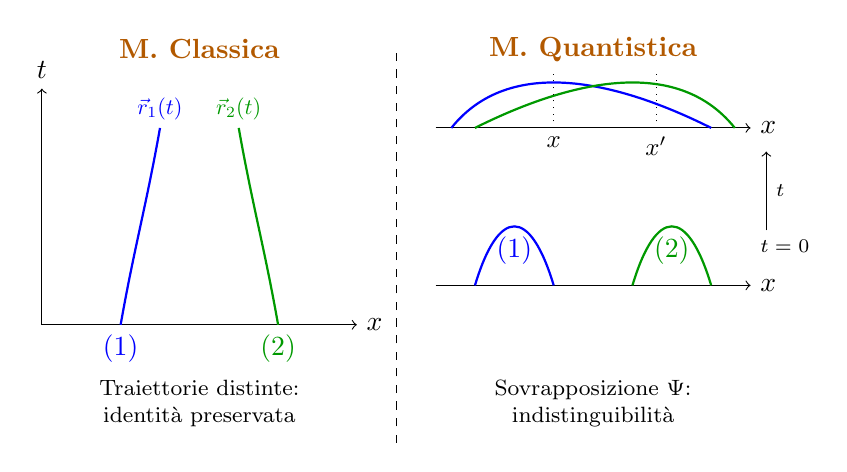
\begin{tikzpicture}
    % Pannello Sinistro: Meccanica Classica
    \begin{scope}[xshift=-4.5cm]
        \node[font=\bfseries, text=orange!70!black] at (2, 3.5) {M. Classica};
        % Assi
        \draw[->] (0,0) -- (4,0) node[right] {$x$};
        \draw[->] (0,0) -- (0,3) node[above] {$t$};
        
        % Traiettorie
        \draw[blue, thick] (1,0) node[below] {(1)} to[out=80, in=260] (1.5,2.5) node[above, scale=0.8] {$\vec{r}_1(t)$};
        \draw[green!60!black, thick] (3,0) node[below] {(2)} to[out=100, in=280] (2.5,2.5) node[above, scale=0.8] {$\vec{r}_2(t)$};
        
        \node[align=center, font=\footnotesize] at (2, -1) {Traiettorie distinte:\\identità preservata};
    \end{scope}

    % Separatore
    \draw[dashed] (0, -1.5) -- (0, 3.5);

    % Pannello Destro: Meccanica Quantistica
    \begin{scope}[xshift=0.5cm]
        \node[font=\bfseries, text=orange!70!black] at (2, 3.5) {M. Quantistica};
        
        % Asse x per t=0
        \draw[->] (0,0.5) -- (4,0.5) node[right] {$x$};
        \node[right] at (4, 1) {\scriptsize $t=0$};
        
        % Pacchetti t=0
        \draw[blue, thick] (0.5,0.5) .. controls (0.8,1.5) and (1.2,1.5) .. (1.5,0.5) node[midway, below] {(1)};
        \draw[green!60!black, thick] (2.5,0.5) .. controls (2.8,1.5) and (3.2,1.5) .. (3.5,0.5) node[midway, below] {(2)};
        
        % Asse x per t > 0
        \draw[->] (0,2.5) -- (4,2.5) node[right] {$x$};
        \draw[->] (4.2, 1.2) -- (4.2, 2.2) node[midway, right] {\scriptsize $t$};
        
        % Pacchetti sovrapposti t > 0
        \draw[blue, thick] (0.2,2.5) .. controls (1,3.5) and (2.5,3) .. (3.5,2.5);
        \draw[green!60!black, thick] (0.5,2.5) .. controls (1.5,3) and (3,3.5) .. (3.8,2.5);
        
        % Punti x e x'
        \draw[dotted] (1.5, 2.5) -- (1.5, 3.2);
        \node[below, scale=0.9] at (1.5, 2.5) {$x$};
        \draw[dotted] (2.8, 2.5) -- (2.8, 3.2);
        \node[below, scale=0.9] at (2.8, 2.5) {$x'$};
        
        \node[align=center, font=\footnotesize] at (2, -1) {Sovrapposizione $\Psi$:\\indistinguibilità};
    \end{scope}
\end{tikzpicture}
\end{center}

% 23 Lezione del 19/11/2025

\lezione{23}{19/11/2025}

Consideriamo ora una particella su uno spazio di Hilbert \(\mathcal{H}\), due insiemi di osservabili I.C.O.C. \(\mathcal{A}\) e \(\mathcal{B}\) e la base di autovettori non degeneri di \(A\) \(\left\{ \ket{a_n} \right\}\).
Se ho due particelle identiche, lo spazio di Hilbert è \(\mathcal{H}\otimes\mathcal{H}= \mathcal{H}^{\otimes2}\) con base ON \(\left\{ \ket{a_{n1}}\otimes \ket{a_{n2}} \right\}\).

Misuriamo \(\mathcal{A}\) su entrambe le particelle, ottenendo due risultati diversi \(a_n\) e \(a_m\). Non sappiamo però su quale particella abbiamo misurato l'uno o l'altro, lo stato dopo la misura sarà dunque:
\[
    \alpha\ket{a_n}\otimes\ket{a_m} + \beta \ket{a_m}\otimes\ket{a_n}
\]
Lo spazio dei vettori compatibile con questa misura ha \(\dim =2\), abbiamo ottenuto della \textit{degenerazione di scambio}.



Consideriamo il caso in cui, dopo aver misurato l'osservabile \( A \), si misuri \( B \). Ci chiediamo quale sia la probabilità che la misura di \( B \) dia due valori diversi per le due particelle \( b_i \neq b_j \).\\
Non sapendo quale sia lo stato del sistema scegliamo arbitrariamente tra \(\ket{a_n}\otimes\ket{a_m} \) e \( \ket{a_m}\otimes\ket{a_n}\).
La probabilità di transizione partendo da uno stato fattorizzato \( \ket{a_n}\otimes\ket{a_m} \) è data dal modulo quadro del prodotto scalare:
\[
    \text{Prob}_{\ket{a_n}\otimes\ket{a_m}}(b_i, b_j) = \abs{(\bra{b_i}\otimes\bra{b_j})(\ket{a_n}\otimes\ket{a_m})}^2
    = \abs{\braket{b_i}{a_n}}^2 \abs{\braket{b_j}{a_m}}^2
\]

Se avessi scelto l'ordine opposto \( \ket{a_m}\otimes\ket{a_n} \), avrei ottenuto:
\[
    \text{Prob}_{\ket{a_m}\otimes\ket{a_n}}(b_i, b_j) = \abs{\braket{b_i}{a_m}}^2 \abs{\braket{b_j}{a_n}}^2
\]

Notiamo che otteniamo probabilità diverse! Quindi le probabilità dipendono dal vettore iniziale scelto. Tuttavia:
\begin{itemize}
    \item Solo una scelta è quella giusta, le altre portano a probabilità sbagliate che non osservo in laboratorio e quindi a risultati teorici errati.
    \item Le particelle sono indistinguibili: le etichette \( (1) \) o \( (2) \) non sono osservabili.
\end{itemize}
Come scegliere, dunque,il vettore iniziale giusto?
Per una particella singola la base è \( \{ \ket{e_n} \} \). Per due particelle lo spazio di Hilbert è il prodotto tensore \( \mathcal{H} \otimes \mathcal{H} = \mathcal{H}^{\otimes 2} \) 
con base \( \{ \ket{e_n}\otimes\ket{e_m} \} \), le nostre teorie devono essere invarianti per lo scambio delle etichette 1 e 2.\\
Formalizziamo meglio questo concetto.

\subsection{Simmetria di Scambio}
Definiamo un operatore unitario su \(\mathcal{H}\) detto \textit{operatore di scambio}:
\begin{equation}
    \hat{P}_{1,2} ( \ket{u}\otimes\ket{v} ) = \ket{v}\otimes\ket{u}
\end{equation}

\textbf{Proprietà:}
\begin{itemize}
    \item Il dominio è \( D(\hat{P}_{12}) = \mathcal{H} \otimes \mathcal{H} \) e l'immagine è \( \hat{P}_{12}(\mathcal{H} \otimes \mathcal{H}) = \mathcal{H} \otimes \mathcal{H} \).
    \item Conserva la norma: \( \norm{\hat{P}_{12}\ket{\Psi}}^2 = \norm{\ket{\Psi}}^2 \).
    \item 
    \(
    \hat{P}_{12}^2 = I \implies \hat{P}_{12} = \hat{P}_{12}^{-1} = \hat{P}_{12}^\dagger \implies \hat{P}_{12} \text{ è a.a.}
    \)
    \item Lo spettro è discreto: \( \sigma(\hat{P}_{12}) = \{ \pm 1 \} \).
\end{itemize}

Possiamo dunque decomporre lo spazio prodotto tensore come somma diretta dei sottospazi relativi agli autovalori:
\[
\mathcal{H}^{\otimes 2} = \mathcal{H}_S \oplus \mathcal{H}_A
\]
dove:
\begin{itemize}
    \item \( \mathcal{H}_S \) (autovalore \( +1 \)): sottospazio simmetrico, \( \hat{P}_{12} \) lascia invariati i vettori qui dentro.
    \item \( \mathcal{H}_A \) (autovalore \( -1 \)): sottospazio antisimmetrico, \( \hat{P}_{12} \) cambia segno ai vettori.
\end{itemize}

\begin{postulato9}
    Dato uno stato fisico rappresentato dal raggio vettore \(\left[ \Psi \right]\), lo scambio di etichette deve lasciare lo stato invariato:
    \begin{equation}
        \left[ \Psi \right]= \left[ \hat{P}_{12} \ket{\Psi}\right]
    \end{equation}
    Dunque: \[
        \hat{P}_{12} \Psi= c_\Psi\ket{\Psi}\,, \ c_\Psi \in \left\{ \pm 1  \right\} \implies \ket{\Psi} \in \mathcal{H}_S \ \text{ o } \ \ket{\Psi} \in \mathcal{H}_A
    \]
\end{postulato9}

\begin{definition}
    Per \(\ket{\Psi} \in \mathcal{H}^{\otimes 2}\) stato fisico di 2 particelle identiche:
    \begin{itemize}
        \item Se \(\ket{\Psi}\in \mathcal{H}_S\), la particella si dice \textit{bosone}.
        \item Se \(\ket{\Psi}\in \mathcal{H}_A\), la particella si dice \textit{fermione}.
    \end{itemize}
\end{definition}

\begin{theorem}
    { \normalfont \textbf{Spin-statistica}}\\
    Una particella di spin \(s \) è un bosone se e solo se \(s \in \mathbb{N}\) o un fermione se e solo se \(s \in \frac{1}{2} + \mathbb{N}\) .
\end{theorem}


Non tutti gli operatori a.a. su \(\mathcal{H}^{\otimes 2}\) corrispondono a un osservabile, un generico operatore \(A = \sum_i B_i\otimes C_i\) definisce un osservabile fisico solo se è invariante per scambio etichette:
\[
    \forall \ket{\Psi} \in \mathcal{H}_S \implies A\ket{\Psi} \in \mathcal{H}_S \qquad 
    \forall \ket{\Psi} \in \mathcal{H}_A \implies A\ket{\Psi} \in \mathcal{H}_A 
\]
\[
    \iff \hat{P}_{12} A \hat{P}^\dagger_{12} = A \iff \left[ A, \hat{P}_{12} \right]=0
\]

\begin{remark}
    Nota che l'azione dell'operatore di scambio sugli operatori tensoriali è data da:
    \[
    \hat{P}_{12} \left( \sum_{i} B_i \otimes C_i \right) \hat{P}_{12}^\dagger = \sum_{i} C_i \otimes B_i
    \]
\end{remark}
\begin{example}
    Se \( B \neq C \), allora:
    \begin{itemize}
        \item \( B \otimes C - C \otimes B \) e \( B \otimes C \) non sono osservabili (perché non simmetrici rispetto allo scambio).
        \item \( B \otimes B \), \( C \otimes C \) e \( B \otimes C + C \otimes B \) sono osservabili.
    \end{itemize}
\end{example}

\begin{remark}
    E' essenziale che anche $H$ sia invariante \quad $\hat{P}_{12} H \hat{P}_{12} = H$\\
    Questa condizione implica che la simmetria (o antisimmetria) dello stato venga preservata durante l'evoluzione temporale:
    \[
    \implies \text{se } \ket{\psi} \in 
    \begin{matrix}
        \mathcal{H}_S \\ \mathcal{H}_A
    \end{matrix} 
    \quad \implies \quad 
    U(t, t_0)\ket{\psi} \in 
    \begin{matrix}
        \mathcal{H}_S \\ \mathcal{H}_A
    \end{matrix}
    \]
\end{remark}

\begin{example}
    Un esempio tipico di Hamiltoniana per due particelle identiche è:
    \[
    H = \frac{\vec{P}_1^2}{2m} + \frac{\vec{P}_2^2}{2m} + V(\vec{X}_1, \vec{X}_2)
    \]
    dove il potenziale di interazione deve essere simmetrico rispetto allo scambio delle coordinate delle particelle:
    \[
    V(\vec{X}_1, \vec{X}_2) = V(\vec{X}_2, \vec{X}_1)
    \]
\end{example}

Grazie al postulato posso risolvere il problema della degenerazione di scambio: se misuro \(A\) su entrambe le particelle e ottengo due risultati \(a_n \neq a_m\), 
l'unica combinazione lineare ammissibile per i bosoni è quella simmetrica:
\begin{equation}
    \frac{1}{\sqrt{2}}\left( \ket{a_n}\otimes\ket{a_m} + \ket{a_n}+ \ket{a_m} \right)  \in \mathcal{H}_S
\end{equation}
Mentre per i fermioni è quella antisimmetrica:
\begin{equation}
    \frac{1}{\sqrt{2}}\left( \ket{a_n}\otimes\ket{a_m} - \ket{a_n}+ \ket{a_m} \right)  \in \mathcal{H}_A
\end{equation}

\begin{attention}
    Cosa succede se le due particelle dovessero trovarsi nello stesso stato \(\Psi \in \mathcal{H}\)? Per i bosoni non è un problema \(\ket{\Psi}\otimes\ket{\Psi} \in \mathcal{H}_S\),
    per i fermioni non esiste una combinazione lineare antisimmetrica!
\end{attention}

\begin{pauli}
    \label{theo: Pauli}
    Se ho due fermioni identici non possono essere nello stesso stato di particella singola.
\end{pauli}


\subsection{Caso N particelle identiche}
Consideriamo uno spazio di Hilbert \(\mathcal{H}^{\otimes N}= \mathcal{H}\otimes...\otimes \mathcal{H}\) con base \(\left\{ \ket{e_{n_1}}\ket{e_{n_2}}...\ket{e_{n_N}} \right\}\) (dove abbiamo omesso il simbolo \(\otimes\) per convenienza), i vettori sono descritti da:
\begin{equation}
    \ket{\Psi} = \sum_{n_1,n_2,...,n_N}c_{n_1,n_2,..., n_N}\ket{e_{n_1}}\ket{e_{n_2}}...\ket{e_{n_N}}
\end{equation}
Vogliamo che la fisica sia invariante per qualsiasi scambio di etichette, cioè permutazioni del tipo:
\begin{equation}
    \pi : \left\{ 1,2,...,N \right\}\to \left\{ 1,2,..., N \right\}
\end{equation}
Consideriamo dunque il gruppo delle permutazioni invertbili \(S_N\) .
\begin{remark}
    Il gruppo \(S_N\) ha \(N!\) elementi ed è non-abeliano se \(N\geq 3\) .
\end{remark}

Per ogni scambio ho un operatore unitario che agisce nel seguente modo:
\begin{align*}
    S_N \ni \pi \rightsquigarrow \hat{P}_{\pi}\ket{\Psi} &=\hat{P}_{\pi} \left( \sum_{n_1, \dots, n_N} c_{n_1, \dots, n_N} \ket{e_{n_1}} \ket{e_{n_2}} \dots \ket{e_{n_N}} \right) \\
    &=\sum_{n_1, \dots, n_N} c_{n_1, \dots, n_N} \ket{e_{n_{\pi^{-1}(1)}}} \ket{e_{n_{\pi^{-1}(2)}}} \dots \ket{e_{n_{\pi^{-1}(N)}}}
\end{align*}

L'azione sui singoli vettori prodotto è quindi:
\[
\hat{P}_{\pi} \ket{u_1} \dots \ket{u_N} = \ket{u_{\pi^{-1}(1)}} \ket{u_{\pi^{-1}(2)}} \dots \ket{u_{\pi^{-1}(N)}}
\]

Ottengo così gli operatori \(\hat{P}_{\pi} \) per cui vale \(\hat{P}_{\pi} \hat{P}_{\pi'}= \hat{P}_{\pi\circ \pi'}\) e \(\hat{P}_{\pi}^\dagger = \hat{P}_{\pi}^{-1}= \hat{P}_{\pi^{-1}} \),
i \(\hat{P}_{\pi} \) sono dunque rapresentazione unitaria non proiettiva di \(S_N\).
\begin{remark}
    Si è definita l'azione di \(\hat{P}_{\pi} \) usando la permutazione inversa \(\pi^{-1}\) perché altrimenti \(\hat{P}_{\pi} \hat{P}_{\pi'}= \hat{P}_{\pi\circ \pi'}\) avrebbe le composizione al contrario e non sarebbe lo stesso gruppo. 
\end{remark}


\begin{postulato9}
    {\normalfont (Caso generale)}\\
    Consideriamo \( N \) particelle identiche, \( \ket{\Psi} \in \mathcal{H}^{\otimes N} \) rappresenta uno stato fisico se e solo se:
    \begin{equation}
        \forall \pi \in S_N \quad \hat{P}_{\pi} \ket{\Psi} = c_{\pi}(\Psi) \ket{\Psi}
    \end{equation}
\end{postulato9}
Si nota che:
\begin{itemize}
        \item Deve valere \( |c_{\pi}(\Psi)| = 1 \).
        \item Se voglio che \( \forall \Psi, \Psi' \) fisici, anche la sovrapposizione \( \Psi + \Psi' \) sia uno stato fisico \( \implies c_{\pi}(\Psi) = c_{\pi}(\Psi') \) (cioè la costante \( c \) non dipende dallo specifico stato \( \Psi \)).
\end{itemize}




Consideriamo un particolare caso di permutazioni, le trasposizioni \(\pi_{ij}\) cambiano solo 2 elementi dell'insieme lasciando invariati gli altri:
\[
\begin{matrix}
1 & \longrightarrow & 1 \\
\vdots & & \vdots \\
i & \longrightarrow & j \\
\vdots & & \vdots \\
j & \longrightarrow & i \\
\vdots & & \vdots \\
N & \longrightarrow & N
\end{matrix}
\]

Qualunque permutazione la ottengo componendo trasposizioni:
\[
\forall \pi \in S_N, \quad \pi = \pi_{i_1 j_1} \circ \pi_{i_2 j_2} \circ \dots \circ \pi_{i_\ell j_\ell}
\]
Da cui segue la scomposizione per gli operatori:
\[
\hat{P}_{\pi} = \hat{P}_{i_1 j_1} \dots \hat{P}_{i_\ell j_\ell}
\]

\begin{remark}
    La decomposizione di una permutazione \( \pi \) in trasposizioni non è unica.
    Ciò implica che il numero di trasposizioni \( \ell \) può essere diverso, ma tutte le decomposizioni avranno la stessa parità.
\end{remark}

\begin{definition}
    Una permutazione \( \pi \) è detta \textit{pari/dispari} se e solo se il numero di trasposizioni \( \ell \) nella sua decomposizione è pari/dispari.
\end{definition}

Essendo gli autovalori di una singola trasposizione \(\left\{ \pm 1 \right\}\) gli unici autovalori possibili per una permutazione sono:

\begin{enumerate}
    \item \( c_{\pi} = +1 \quad \forall \pi \in S_N \)
    \item \( c_{\pi} = \mathrm{Sgn}(\pi) = 
    \begin{cases}
        +1 & \text{se } \pi \text{ è pari} \\
        -1 & \text{se } \pi \text{ è dispari}
    \end{cases}
    \)
\end{enumerate}


\begin{theorem}
    { \normalfont \textbf{Spin-statistica}}\\
    \(N\) particelle identiche sono bosoni \(s \in \mathbb{N}\) se e solo se:
    \begin{equation}
        \hat{P}_{\pi}\ket{\Psi}= +\ket{\Psi} \quad  \forall\,\pi \in S_N \iff \ket{\Psi}\in \mathcal{H}_S \subseteq \mathcal{H}^{\otimes N}
    \end{equation}
    \(N\) particelle identiche sono fermioni \(s \in \frac12 + \mathbb{N}\) se e solo se:
    \begin{equation}
        \hat{P}_{\pi}\ket{\Psi}= \mathrm{Sgn}(\pi)\ket{\Psi} \quad  \forall\,\pi \in S_N \iff \ket{\Psi}\in \mathcal{H}_A \subseteq \mathcal{H}^{\otimes N}
    \end{equation}
\end{theorem}

\begin{remark}
    \(\mathcal{H}^{\otimes N}= \mathcal{H}_S \oplus \mathcal{H}_A \oplus \dots\) le altre componenenti sono spazi di Hilbert di stati non fisici.
\end{remark}

% 24 Lezione del 21/11/2025

\begin{example}
    \textbf{\(N=3\)}\\
    \lezione{24}{21/11/2025}
    Analizziamo la costruzione degli stati fisici per un sistema di 3 particelle identiche a partire dagli stati di singola particella.
    Per particelle bosoniche gli stati devono essere completamente simmetrici sotto scambio di particelle, ovvero invarianti per ogni permutazione \(\pi\).
    \begin{itemize}
        \item \textbf{3 particelle nello stesso stato \(\ket{u}\):}
        \[
            \ket{u}\otimes\ket{u}\otimes\ket{u} = \ket{u}\ket{u}\ket{u}
        \]
        Questo stato è già invariante per qualsiasi permutazione, quindi appartiene a \(\mathcal{H}_S\).

        \item \textbf{2 particelle in \(\ket{u}\) e 1 in \(\ket{v}\):}
        Preso singolarmente, \(\ket{u}\ket{u}\ket{v}\) non è uno stato fisico per particelle indistinguibili. Dobbiamo costruire una combinazione lineare simmetrica sommando le permutazioni distinte:
        \[
            \frac{1}{\sqrt{3}}\left( \ket{u}\ket{u}\ket{v} + \ket{u}\ket{v}\ket{u} + \ket{v}\ket{u}\ket{u} \right) \in \mathcal{H}_S
        \]
        dove \(\frac{1}{\sqrt{3}}\) è il fattore di normalizzazione.

        \item \textbf{3 particelle in stati tutti diversi \(\ket{a}, \ket{b}, \ket{c}\):}
        Per ottenere una combinazione simmetrica appartenente a \(\mathcal{H}_S\), dobbiamo sommare su tutte le permutazioni possibili (\(3! = 6\)):
        \[
            \frac{1}{\sqrt{6}}\Big( \ket{a}\ket{b}\ket{c} + \ket{b}\ket{c}\ket{a} + \ket{c}\ket{a}\ket{b} + \ket{b}\ket{a}\ket{c} + \ket{a}\ket{c}\ket{b} + \ket{c}\ket{b}\ket{a} \Big) \in \mathcal{H}_S
        \]
        In generale, otteniamo lo stato fisico sommando sulle permutazioni \(\pi \in S_N\) tramite l'operatore di permutazione \(\hat{P}_\pi\):
        \[
            \mathcal{N} \sum_{\pi \in S_N} \hat{P}_\pi \ket{a}\ket{b}\ket{c} \in \mathcal{H}_S
        \]
    \end{itemize}

    Se vogliamo rappresentare dei fermioni, lo stato deve essere totalmente antisimmetrico e appartenere a \(\mathcal{H}_A\). La somma diventa una somma alternante, con segno positivo per le permutazioni pari e negativo per quelle dispari:
    \[
        \frac{1}{\sqrt{6}}\Big( \ket{a}\ket{b}\ket{c} + \ket{b}\ket{c}\ket{a} + \ket{c}\ket{a}\ket{b} - \ket{b}\ket{a}\ket{c} - \ket{a}\ket{c}\ket{b} - \ket{c}\ket{b}\ket{a} \Big) \in \mathcal{H}_A
    \]
    La formula generale coinvolge la segnatura della permutazione \(\operatorname{sgn}(\pi)\):
    \[
        \mathcal{N} \sum_{\pi \in S_N} \operatorname{sgn}(\pi) \hat{P}_\pi \ket{a}\ket{b}\ket{c} \in \mathcal{H}_A
    \]
    \begin{attention}
        Se avessimo due stati uguali (ad esempio \(\ket{a} = \ket{b}\)), i termini con segno opposto si cancellerebbero a vicenda annullando l'intera somma.
        Questo risultato costituisce l'estensione del \textit{Principio di esclusione di Pauli} ( \ref{theo: Pauli}): non possono esserci due fermioni nello stesso stato quantico.
    \end{attention}
\end{example}

\subsubsection{Osservabili fisici}
Le osservabili fisiche sono rappresentate da operatori autoaggiunti \(A: \mathcal{H}^{\otimes N} \to \mathcal{H}^{\otimes N}\) che commutano con ogni operatore di permutazione:
    \begin{equation}
        [A, \hat{P}_\pi] = 0 \quad \forall \pi \in S_N
    \end{equation}
    Questa condizione è equivalente a richiedere che l'operatore sia invariante sotto coniugazione per una qualsiasi permutazione:
    \begin{equation}
        \hat{P}_\pi A \hat{P}_\pi^\dagger = A \quad \forall \pi \in S_N
    \end{equation}
In particolare, questa proprietà deve valere per l'operatore Hamiltoniano del sistema:
    \begin{equation}
        \hat{P}_\pi H \hat{P}_\pi^\dagger = H \quad \forall \pi \in S_N
    \end{equation}

\begin{attention}
    Le osservabili devono essere sempre \textbf{simmetriche} rispetto allo scambio di particelle, a differenza degli stati (che possono essere antisimmetrici nel caso dei fermioni).
\end{attention}

\begin{example}
    Consideriamo un esempio con 3 particelle e due operatori di singola particella \(A\) e \(B\). Vogliamo costruire un operatore globale simmetrico.
    La combinazione:
    \[
        \mathcal{O} = A\otimes A \otimes B + A\otimes B \otimes A + B\otimes A \otimes A
    \]
    è corretta. Se, per esempio, agisco con l'operatore di permutazione \(\hat{P}_{23}\) (scambio tra la particella 2 e 3):
    \begin{itemize}
        \item \(A\otimes \mathbf{A} \otimes \mathbf{B} \xrightarrow{\hat{P}_{23}} A\otimes \mathbf{B} \otimes \mathbf{A}\)
        \item \(A\otimes \mathbf{B} \otimes \mathbf{A} \xrightarrow{\hat{P}_{23}} A\otimes \mathbf{A} \otimes \mathbf{B}\)
        \item \(B\otimes \mathbf{A} \otimes \mathbf{A} \xrightarrow{\hat{P}_{23}} B\otimes \mathbf{A} \otimes \mathbf{A}\)
    \end{itemize}
    Se permuto gli elementi, la somma totale rimane uguale, quindi l'operatore è simmetrico.
\end{example}

\subsection{Sistema a due elettroni e composizione degli spin}

Consideriamo un sistema composto da 2 elettroni ($2\,e^-$). Lo spazio di Hilbert totale è il prodotto tensore degli spazi delle singole particelle:
\begin{itemize}
    \item Spazio di Hilbert della 1° particella: \(\mathcal{H}_1 = \mathcal{H}_{\vec{x}_1} \otimes \mathcal{H}_{s_1}\)
    \item Spazio di Hilbert della 2° particella: \(\mathcal{H}_2 = \mathcal{H}_{\vec{x}_2} \otimes \mathcal{H}_{s_2}\)
\end{itemize}
Per comodità, possiamo raggruppare la parte spaziale e la parte di spin:
\[
    \mathcal{H}^{tot} = (\mathcal{H}_{\vec{x}_1} \otimes \mathcal{H}_{s_1}) \otimes (\mathcal{H}_{\vec{x}_2} \otimes \mathcal{H}_{s_2}) 
    \cong \underbrace{(\mathcal{H}_{\vec{x}_1} \otimes \mathcal{H}_{\vec{x}_2})}_{\mathcal{H}^{pos}} \otimes \underbrace{(\mathcal{H}_{s_1} \otimes \mathcal{H}_{s_2})}_{\mathcal{H}^{spin}}
\]
Dove:
\begin{itemize}
    \item \(\mathcal{H}^{pos} \cong L_2(\mathbb{R}^3 \times \mathbb{R}^3, d^3x_1 d^3x_2)\)
    \item \(\mathcal{H}^{spin} \cong \mathbb{C}^2 \otimes \mathbb{C}^2\) (dimensione totale \(2\times2=4\))
\end{itemize}

Come già visto abbiamo due possibili scelte per l'insieme completo di osservabili che commutano (I.C.O.C.):
\begin{itemize}
    \item Utilizzando gli spin individuali.
    \[
        \{\vec{X}_1, \vec{X}_2, S_{1z}, S_{2z}\} \quad \longrightarrow \quad \ket{\vec{x}_1, \vec{x}_2, m_1, m_2}
    \]
    
    \item Utilizzando lo spin totale del sistema \(\vec{S} = \vec{S}_1 + \vec{S}_2\).
    \[
        \{\vec{X}_1, \vec{X}_2, \vec{S}^2, S_z\} \quad \longrightarrow \quad \ket{\vec{x}_1, \vec{x}_2, S, m}
    \]
\end{itemize}

\subsubsection{Stati di Singoletto e Tripletto}
Effettuiamo il cambio di base per la parte di spin. Avendo \(s_1 = 1/2\) e \(s_2 = 1/2\), lo spin totale \(S\) può assumere valori nell'intervallo \(|s_1 - s_2| \le S \le s_1 + s_2\), ovvero \(S \in \{1, 0\}\).
I 4 stati possibili si raggruppano in:

\paragraph{Tripletto (\(S=1\))}
Spin totale del sistema \(1\), simmetrico per scambio. Ci sono 3 stati (\(m=1, 0, -1\)):
\begin{equation}
    \begin{cases}
        \ket{1, 1} = \ket{+ +} \\
        \ket{1, 0} = \frac{1}{\sqrt{2}} \left( \ket{+ -} + \ket{- +} \right) \\
        \ket{1, -1} = \ket{- -}
    \end{cases}
\end{equation}
Lo stato \(\ket{1,0}\) si ottiene applicando l'operatore di abbassamento \(S_-\) allo stato \(\ket{1,1}\).

\paragraph{Singoletto (\(S=0\))}
Spin totale nullo, antisimmetrico per scambio. C'è un solo stato (\(m=0\)), che deve essere ortogonale a \(\ket{1,0}\):
\begin{equation}
    \ket{0, 0} = \frac{1}{\sqrt{2}} \left( \ket{+ -} - \ket{- +} \right)
\end{equation}
Questo stato appare solo una volta poiché \(S\) ha un solo valore disponibile (\(s_1 - s_2 = 0\)).

Uno stato generico \(\ket{\Psi}\) in \(\mathcal{H}^{\otimes 2}\) può essere scritto espandendo sulla base accoppiata:
\begin{equation}
    \ket{\Psi} = \sum_{S=0}^{1} \sum_{m=-S}^{S} \Psi_{S,m}(\vec{x}_1, \vec{x}_2) \ket{S, m}
        \equiv \sum_{S,m} \Psi_{S,m}(\vec{x}_1, \vec{x}_2) \otimes \ket{S, m}
\end{equation}
dove le \(\Psi_{S,m}(\vec{x}_1, \vec{x}_2) = \braket{\vec{x}_1, \vec{x}_2, S, m}{\Psi}\) sono 4 funzioni d'onda spaziali che specificano lo stato.

Poiché sono fermioni, la funzione d'onda totale $\ket{\Psi}$ deve essere antisimmetrica rispetto allo scambio delle particelle. Definito l'operatore di scambio $\hat{P}_{12}$, deve valere:
\[
    \hat{P}_{12} \ket{\Psi} = - \ket{\Psi}
\]

L'operatore di scambio agisce sia sui gradi di libertà spaziali che su quelli di spin. Possiamo scriverlo come prodotto tensore:
\[
    \hat{P}_{12} = \hat{P}_{12}^{pos} \otimes \hat{P}_{12}^{spin}
\]

Analizziamo l'azione separata delle due componenti:
\begin{itemize}
    \item \textbf{Parte spaziale:} scambia le coordinate delle due particelle:
    \[
    \hat{P}_{12}^{pos} \Psi(\vec{x}_1, \vec{x}_2) = \Psi(\vec{x}_2, \vec{x}_1)
    \]
    \item \textbf{Parte di spin:} scambia i numeri quantici di spin $m_1$ e $m_2$:
    \[
    \hat{P}_{12}^{spin} \ket{m_1, m_2} = \ket{m_2, m_1}
    \]
\end{itemize}


L'azione di $\hat{P}_{12}^{spin}$ dipende dallo stato di spin totale $S$ del sistema:
\begin{itemize}
    \item Per lo stato di \textbf{Tripletto} ($S=1$), lo stato è simmetrico per scambio:
    \[
    \hat{P}_{12}^{spin} \ket{1, m} = + \ket{1, m}
    \]
    \item Per lo stato di \textbf{Singoletto} ($S=0$), lo stato è antisimmetrico per scambio:
    \[
    \hat{P}_{12}^{spin} \ket{0, 0} = - \ket{0, 0}
    \]
\end{itemize}

Imponiamo ora la condizione che lo stato fisico complessivo sia antisimmetrico:
\[
    \hat{P}_{12} \ket{\Psi_{S,m}} = \left( \hat{P}_{12}^{pos} \otimes \hat{P}_{12}^{spin} \right) \left( \Psi_{space} \otimes \ket{S,m} \right) = - \ket{\Psi_{S,m}}
\]
Affinché il totale sia negativo, le simmetrie spaziali e di spin devono essere opposte.


Per lo stato di tripleto (\(s=1\)), la parte di spin è simmetrica ($+$). Di conseguenza, la parte spaziale deve essere \textbf{antisimmetrica} ($-$) per ottenere un segno totale negativo:
\[
    \implies \Psi_{S=1, m}(\vec{x}_2, \vec{x}_1) = - \Psi_{S=1, m}(\vec{x}_1, \vec{x}_2)
\]

Invece per lo stato di singoletto (\(s=0\)), la parte di spin è antisimmetrica ($-$). Di conseguenza, la parte spaziale deve essere \textbf{simmetrica} ($+$):
\[
    \implies \Psi_{S=0, 0}(\vec{x}_2, \vec{x}_1) = + \Psi_{S=0, 0}(\vec{x}_1, \vec{x}_2)
\]

\subsubsection{Effetto fisico di funzioni d'onda simmetirce e antisimmetriche}

Consideriamo due funzioni d'onda di particella singola \(\psi_A(\vec{x}), \psi_B(\vec{x}) \in L_2(\mathbb{R}^3)\), con \(\psi_A \neq \psi_B\):
\begin{equation}
    \int \abs{\psi_{A,B}(\vec{x})}^2 \dd[3]{x} = 1 \qquad \braket{\psi_A}{\psi_B} = 0
\end{equation}

Supponiamo di avere due \(e^-\), uno con funzione d'onda \(\psi_A\) e uno con funzione d'onda \(\psi_B\) (e qualche stato di spin). 
La funzione d'onda spaziale totale sarà:
\begin{equation}
    \Psi_{\substack{S=0 \\ S=1}} (\vec{x}_1, \vec{x}_2) = \frac{1}{\sqrt{2}} \left( \psi_A(\vec{x}_1) \psi_B(\vec{x}_2) \pm \psi_A(\vec{x}_2) \psi_B(\vec{x}_1) \right)
\end{equation}
Il più per le funzioni d'onda simmetriche e il meno per le funzioni d'onda antisimmetriche. Entrambe le funzioni sono normalizzate:
\[
    \int \abs{\Psi(\vec{x}_1, \vec{x}_2)}^2 \dd[3]{x_1} \dd[3]{x_2} = 1
\]

Calcoliamo la probabilità di trovare entrambe le particelle nella stessa posizione \(\vec{x}_1 = \vec{x} = \vec{x}_2\):
\begin{equation}
    \rho(\vec{x}, \vec{x}) = \abs{\Psi(\vec{x}, \vec{x})}^2
\end{equation}

Analizziamo i tre casi possibili:

\begin{enumerate}
    \item \textbf{\(\Psi\) simmetrica}:
    \begin{equation}
        \rho_S(\vec{x}, \vec{x}) = \abs{\frac{1}{\sqrt{2}} \left( 2\psi_A(\vec{x})\psi_B(\vec{x}) \right)}^2 = \frac{1}{2} \cdot 4 \abs{\psi_A(\vec{x})}^2 \abs{\psi_B(\vec{x})}^2 = 2 \abs{\psi_A(\vec{x})}^2 \abs{\psi_B(\vec{x})}^2
    \end{equation}
    La probabilità è doppia rispetto al caso di particelle distinguibili (attrazione efficace).

    \item \textbf{\(\Psi\) antisimmetrica}:
    \begin{equation}
        \rho_A(\vec{x}, \vec{x}) = \abs{\frac{1}{\sqrt{2}} \left( \psi_A(\vec{x})\psi_B(\vec{x}) - \psi_A(\vec{x})\psi_B(\vec{x}) \right)}^2 = 0
    \end{equation}
    La probabilità è nulla: principio di esclusione di Pauli (repulsione efficace).

    \item \textbf{Particelle distinguibili}:
    \begin{equation}
        \Psi_D(\vec{x}_1, \vec{x}_2) = \psi_A(\vec{x}_1)\psi_B(\vec{x}_2)\implies 
            \rho_D(\vec{x}, \vec{x}) = \abs{\psi_A(\vec{x})}^2 \abs{\psi_B(\vec{x})}^2
    \end{equation}
\end{enumerate}

Calcoliamo ora invece la probabilità che le particelle si trovino in posizioni differenti \(\vec{x}\neq \vec{x}'\):

\begin{enumerate}
    \item \textbf{\(\Psi\) Simmetrica o Antisimmetrica (Indistinguibili)}:
    Poiché \(\Psi\) è (anti)simmetrica, il modulo quadro è invariante per lo scambio delle coordinate:
    \begin{equation}
        \abs{\Psi(\vec{x}, \vec{x}')}^2 = \abs{\Psi(\vec{x}', \vec{x})}^2
    \end{equation}
    Quindi la densità totale diventa:
    \[
        \rho_{S,A}^{tot}(\vec{x}, \vec{x}') = 2 \cdot \abs{\Psi(\vec{x}, \vec{x}')}^2 = 2 \cdot \frac{1}{2} \abs{\psi_A(\vec{x})\psi_B(\vec{x}') \pm \psi_A(\vec{x}')\psi_B(\vec{x})}^2
    \]
    Espandendo il modulo quadro:
    \[
        = \abs{\psi_A(\vec{x})}^2 \abs{\psi_B(\vec{x}')}^2 + \abs{\psi_A(\vec{x}')}^2 \abs{\psi_B(\vec{x})}^2 \pm 2 \Re\left( \psi_A^*(\vec{x})\psi_B^*(\vec{x}')\psi_A(\vec{x}')\psi_B(\vec{x}) \right)
    \]
    Il termine aggiuntivo:
    \begin{equation}
        \pm 2 \Re\left( \psi_A^*(\vec{x})\psi_B^*(\vec{x}')\psi_A(\vec{x}')\psi_B(\vec{x}) \right)
    \end{equation}
    rappresenta l'\textbf{interazione di scambio}.

    \item \textbf{Particelle Distinguibili}:
    Per particelle classiche o distinguibili, non c'è simmetrizzazione:
    \begin{equation}
        \rho_D^{tot}(\vec{x}, \vec{x}') = \abs{\psi_A(\vec{x})}^2 \abs{\psi_B(\vec{x}')}^2 + \abs{\psi_A(\vec{x}')}^2 \abs{\psi_B(\vec{x})}^2
    \end{equation}
\end{enumerate}

\begin{example}
    Se abbiamo un \(e^-\) sulla Terra e un altro sulla Luna, devo anti-simmetrizzare il loro stato?

Siano \(\psi_A(\vec{x})\) a supporto in \(R_A\) (Terra) e \(\psi_B(\vec{x})\) a supporto in \(R_B\) (Luna), tali che \(R_A \cap R_B = \emptyset\).
\[
    \psi_{A,B}(\vec{x}) = 0 \quad \forall \vec{x} \notin R_{A,B}
\]

Verifichiamo la probabilità che si trovino nello stesso punto:
\[
    \rho(\vec{x}, \vec{x}) \propto \abs{\psi_A(\vec{x})}^2 \abs{\psi_B(\vec{x})}^2 = 0 \quad \forall \vec{x}
\]
Infatti:
\begin{itemize}
    \item Se \(\vec{x} \in R_A \implies \psi_B(\vec{x}) = 0\)
    \item Se \(\vec{x} \in R_B \implies \psi_A(\vec{x}) = 0\)
    \item Se \(\vec{x} \notin R_A \cup R_B \implies \psi_{A,B}(\vec{x}) = 0\)
\end{itemize}

Il termine di interferenza (scambio) si annulla identicamente:
\[
    2\Re \left( \psi_A^*(\vec{x})\psi_B^*(\vec{x}') \psi_A(\vec{x}')\psi_B(\vec{x}) \right) = 0 \quad \forall \vec{x}, \vec{x}'
\]
Questo perché per ogni coppia \((\vec{x}, \vec{x}')\), almeno uno dei fattori nel prodotto incrociato è nullo (non c'è sovrapposizione delle funzioni d'onda).

\[
    \rho_S^{tot}(\vec{x}, \vec{x}') = \rho_A^{tot}(\vec{x}, \vec{x}') = \rho_D^{tot}(\vec{x}, \vec{x}')
\]
Non commetto alcun errore se le tratto come particelle \textbf{distinguibili}.
\end{example}

